\documentclass[fontsize=12pt,a4paper,final]{scrartcl}[2003/01/01]
\usepackage[ngerman]{babel} 
\usepackage[T1]{fontenc}
\usepackage[utf8]{inputenc} 
\usepackage{float}
\usepackage{listings}
\usepackage{color}
\usepackage{hyperref}
\usepackage{tabularx}
\usepackage[toc,page]{appendix}
\usepackage[style=numeric,backend=bibtex]{biblatex}
\bibliography{Literaturverzeichnis}
\setlength{\parindent}{0pt}

\definecolor{pblue}{rgb}{0.13,0.13,1}
\definecolor{pgreen}{rgb}{0,0.5,0}
\definecolor{pred}{rgb}{0.9,0,0}
\definecolor{pgrey}{rgb}{0.46,0.45,0.48}

\lstset{language=Java,
  basicstyle=\tt,
  breakatwhitespace=false,
  breaklines=true,    
  captionpos=b,
  extendedchars=true, 
  frame=single,  
  numbers=left,
  keywordstyle=\bf,
  showspaces=false,
  showstringspaces=false,  
  showtabs=false,  
  tabsize=2,
  commentstyle=\color{pgreen},
  keywordstyle=\color{pblue},
  stringstyle=\color{pred}
}

\newcommand\todo[1]{\textcolor{red}{#1}}

\title{Robotik Dokumentation - Team Robofreunde n.V.}
\author{Lohr, Schramm, Stumpf, Weber, Wurth}

\date{\today}

%Bilder scalen, wenn größer als Seite
\usepackage[final]{graphicx}
\makeatletter
\def\ScaleIfNeeded{%
	\ifdim\Gin@nat@width>\linewidth
		\linewidth
	\else
		\Gin@nat@width
	\fi
}
\makeatother

\begin{document}

\maketitle
\tableofcontents

\section{Einleitung}\label{se:Einleitung}
\textit{Verfasser: Stumpf}\\
\\
Die Lehrveranstaltung Robotik im SS-2015 hatte die Programmierung des NAO -- eines humanoiden Roboters von Aldebaran -- als übergreifendes Thema. Diesem sollten für Fussball notwendige Bewegungsabläufe und Taktiken beigebracht werden. Aufgrund des großen Andrangs konnten sich nicht alle Teilnehmer mit dem einzigen zur Verfügung stehenden NAO Modell beschäftigen. Die Gruppe wurde also in ein Hardware und 2 Simulationsteams aufgeteilt.\\
\\
Die vorgegebene Simulationumgebung war die auf Simspark basierende RoboCup 3D-Soccer Simulation League.\\
Das Ziel unserer beiden Simulationsteams war es, je eine eigene Mannschaft aufs Feld zu bringen und diese am Ende gegeneinander antreten zu lassen.\\
\\
RoboCup ist eine Fussball-Liga humanoider Roboter. Die Teams mehrerer Länder treten gegeneinander an, um ein bestes Team zu ermitteln. In der RoboCup Soccer Simulation League werden die Spiele simuliert. Die Roboter werden durch virtuelle Instanzen ersetzt, die über definierte Schnittstellen auf den Server verbunden und gesteuert werden können.\\
\\
Es gibt eine 2D und eine 3D Version. Für uns war insbesondere die 3D Version interessant, weil NAO hier das aktuelle Robotermodell ist. Anforderungen und Regeln der 3D Version sind vergleichbar mit dem echten RoboCup. Das Regelwerk möchte soll hier nicht noch einmal näher erläutern werden, es ist auf \\
\href{www.robocupgermanopen.de/sites/default/files/rules_GO_2015_3DSim.pdf}{www.robocupgermanopen.de/sites/default/files/rules\_GO\_2015\_3DSim.pdf} sehr gut beschrieben.\\
\\
Da die Schnittstellen zum Server auf sehr niedriger Ebene definiert sind (Bewegung von Gelenken), ist es für den Zeitraum der Lehrveranstaltung zu aufwändig, einen virtuellen Roboter komplett selbstständig zu entwickeln. Es gibt allerdings einige Frameworks, auf denen die eigene Arbeit aufgebaut werden kann.

\section{Anforderungen}
\textit{Verfasser: Weber}\\
\\

Es gab nur einige wenige Anforderungen, welche folgend dokumentiert werden.

\begin{itemize}
\item Bis zum Ende des Semsters soll eine funktionierende RoboCup Mannschaft im Team entwickelt werden
\item Die entwickelte Mannschaft soll in der 3D Umgebung des RoboCups agieren
\item Am Ende des Semester soll ein Spiel zwischen den beiden Studenten-Teams durchgeführt werden
\end{itemize}

\section{Zeitplan}
\textit{Verfasser: Stumpf, Schramm, Wurth, Weber}\\
\\
Die folgende Timeline soll ein Überblick über den Verlauf der Lehrveranstaltung geben und insbesondere die Frage \textit{\glqq Wann wurde was gemacht?\grqq} beantworten.

\begin{figure}[H]
	\centering
	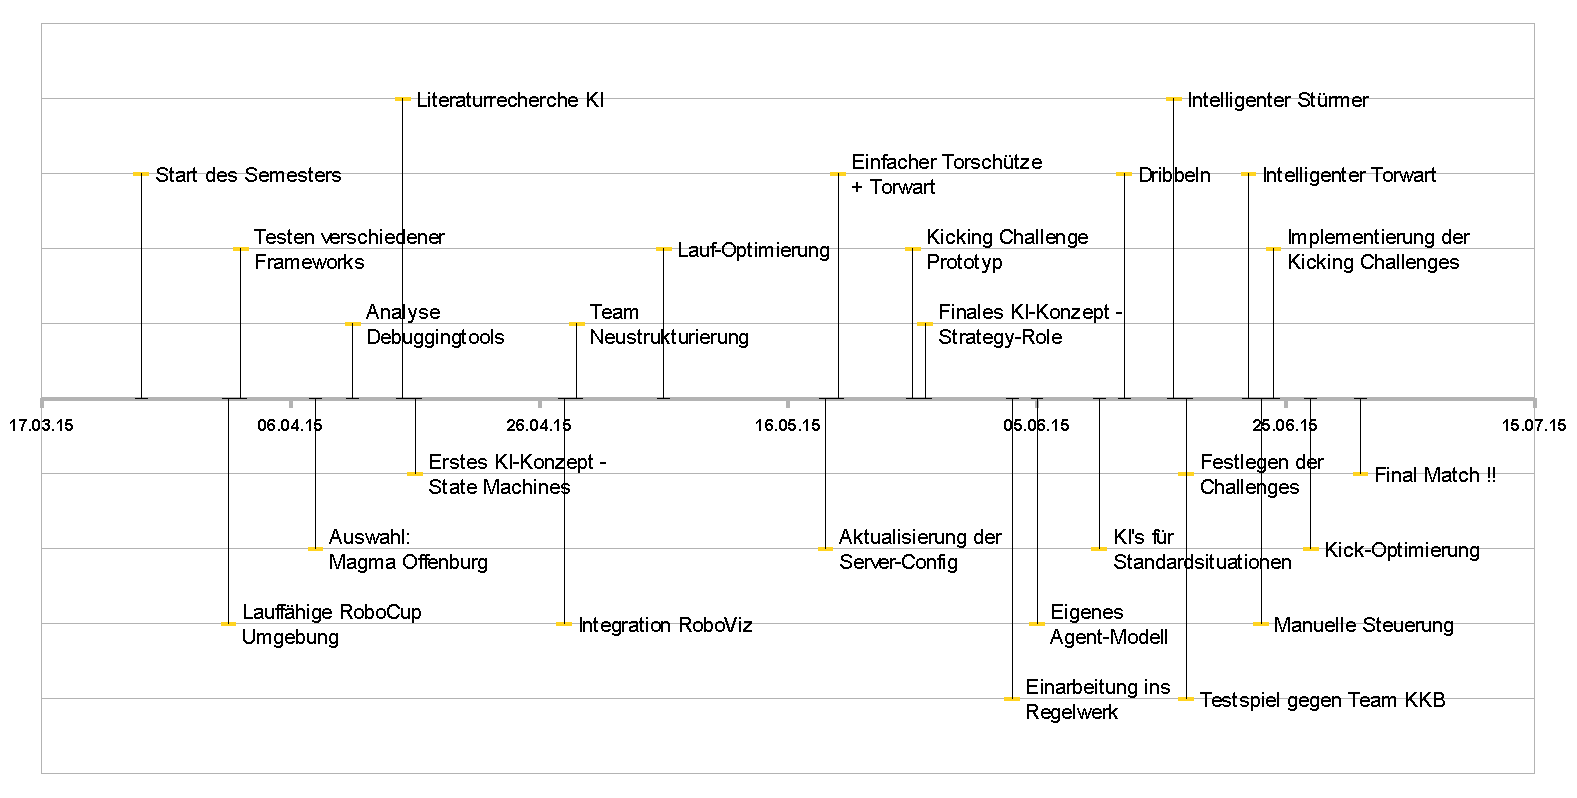
\includegraphics[width=\textwidth]{Grafiken/Timeline_cropped}
	\caption{Team Robofreunde - Timeline}
	\label{fig:Timeline}
\end{figure}

\section{RoboCup Soccer Simulation League}
\textit{Verfasser: Stumpf}\\
\\
Simspark ist die Engine, auf der der die RoboCup Soccer Simulation League aufgebaut ist. Es wird als generisches Simulationssystem für mehrere Agents beschrieben und ist bei Sourceforge als OpenSource Projekt registriert.\\
\\
In der RoboCup Simulation können sich die Agents -- NAO-Agents in 3D -- mit dem Server verbinden und über ein Textprotokoll mit diesem kommunizieren. In jedem Zyklus werden vom NAO-Agent Daten über die gewünschten Bewegungen der Effektoren (Gelenke) an den Server gesendet, der den virtuellen NAO entsprechend reagieren lässt. Als Antwort erhält der Agent Informationen über die Position seiner Effektoren und Daten seiner Sensoren (z.B. visuelle Sensoren, Lagesensoren).\\
\\
Die erste Herausforderung war es, die Simulationsumgebung lokal auf jedem der Rechner zu installieren, um Entwicklung und Tests zu ermöglichen. Unsere Erfahrungen werden in diesem Abschnitt kurz zusammengefasst. Für das Endspiel wurde uns ein Rechner für die Installation des Servers zur Verfügung gestellt. Diese Aufgabe hat das andere Simulations-Team übernommen.\\
\\
Installationsanleitungen für verschiedene Systeme findet man im Wiki von Simspark auf \href{http://simspark.sourceforge.net/wiki/index.php/Main_Page}{http://simspark.sourceforge.net/wiki/index.php/Main\_Page}.\\
\\
Die benötigten Komponenten sind der Simulationsserver - rcssserver3d sowie der Monitor - rcssmonitor3d, der das Spielgeschehen grafisch darstellt. Die von uns verwendete Server Version ist v6.8.1.

\subsection{Installation auf Windows Systemen}
\textit{Verfasser: Stumpf}\\
\\
Trotz wiederholter Versuche von Teammitgliedern beider Teams haben wir die zu unserem Zeitpunkt zur Verfügung stehende Windows Version 6.7 nicht nicht zum Laufen gebracht. 
\subsection{Installation Linux Systemen}
\textit{Verfasser: Stumpf}\\
\\
Sowohl auf ArchLinux und Debian ist die Simulationsumgebung lauffähig. Die Installation muss auf diesen Systemen allerdings manuell über das zur Verfügung stehende tar.gz erfolgen.\\
\\
Auf Fedora hingegen funktioniert die Installation sehr komfortabel, da die Pakete im Paketmanager hinterlegt sind via \texttt{'yum install rcssserver3d'}.
\subsection{Installation Windows + VM}
\textit{Verfasser: Stumpf}\\
\\
Um auf Windows Systemen dennoch entwickeln und testen zu können, haben wir eine VM mit Fedora aufgesetzt (z.B. Virtual Box) und auf dieser die Simulationsumgebung installiert. Es ist darauf zu achten, einen Netzwerkadapter als Host-Only Adapter einzurichten, um auf den Server zugreifen zu können.\\
\\
In Kombination mit RoboViz (siehe \autoref{se:Grafisches Debugging}) ist es möglich, nur noch den rcssserver3d in der VM zu starten, da der RoboViz Monitor problemlos auf Windows läuft.

\section{Framework}
\textit{Verfasser: Stumpf}\\
\\
Für die Entwicklung von Agents für die RoboCup Soccer Simulation League wird auf der Wiki Seite von Simspark eine Vielzahl von Frameworks vorgestellt. Nach Evaluation dieser stellt sich jedoch heraus, dass viele davon nicht mehr als ein grobes Gerüst für die Kommunikation mit dem Server, schlecht bis gar nicht dokumentiert oder seit Jahren nicht mehr gepflegt und damit inkompatibel zur aktuellen Server Version sind.\\
\\
Die Frameworks, die nach näherer Untersuchung noch in Betracht kamen waren:
\begin{itemize}
\item Magma Offenburg (Java)
\item libbats (c++)
\item tinman (c\#)
\item Zigorat (c++)
\end{itemize}

\subsection{Entscheidung für Magma}
\textit{Verfasser: Stumpf}\\
\\
Folgende Punkte haben wir in einer Diskussionsrunde als Grundlage für die Entscheidung des Frameworks festgelegt:
\begin{itemize}
\item Umsetzung der Grundbewegungen soll vorhanden sein. Dazu zählen:
	\begin{itemize}
	\item Gehen/Laufen
	\item Aufstehen
	\item Schie{\ss}en
	\end{itemize}
\item Gute Dokumentation, vorzugsweise in englisch.
\item Programmiersprache sollte allen Gruppenmitgliedern bekannt sein. 
\item Das Framework sollte aktuell sein und noch gepflegt werden.
\item Ein Worldmodel, welches Informationen über Spielzustand, Spieler auf dem Feld u.a. enthält, ist erwünscht.
\item Beispielimplementierung eines Agents vorhanden.
\end{itemize}

Nach dem Ausscheiden der offensichtlich ungeeigneten Kandidaten haben wir uns letztendlich für Magma Offenburg entschieden. Grundlage für die Entscheidung war, dass Magma unsere obigen Anforderungen nahezu gänzlich erfüllt hat. Das einzige Manko, welches aber erst später in der Entwicklung deutlicher wurde, ist die Dokumentation. Essenzielle Methoden sind zum Teil gar nicht, falsch oder unzureichend mit JavaDoc versehen.

Im Vergleich zu den anderen Kandidaten ausschlaggebend war unter anderem:
\begin{itemize}
\item Die Programmiersprache Java kam den meisten unserer Gruppenmitglieder sehr gelegen. In Absprache mit der anderen Simulationsgruppe wurde au{\ss}erdem dafür gestimmt, unterschiedliche Sprachen zu verwenden. Ein weiterer Grund.
\item Magma Offenburg bietet mehrere Schussimplementierungen, was zumindest tinman und libbats nicht vorweisen können.
\item Die Trennung der Agents in logische Abstraktionsebenen, DecisionMaker (Trifft Entscheidung was zu tun ist), Belief (Gibt zurück ob ein Zustand zutrifft, z.B. "Liege ich am Boden?"), Behavior (Führt aus was zu tun ist) war uns sympathisch.
\end{itemize}

Hier noch einmal ein Überblick über Vorteile und Nachteile von Magma Offenburg:
\\

\begin{tabularx}{\textwidth}{|X|X|}
\hline
 \textbf{Vorteile}&\textbf{Nachteile}\\
\hline
\hline
 Großer Funktionsumfang&Großer Umfang, komplex\\
\hline 
 Java&Gewachsene Struktur, unübersichtlich, viele nicht verwendete Klassen und Methoden\\
\hline
 Abstraktionsebenen&Viele Abhängigkeiten, Änderung an A -> Änderung an B notwendig\\
\hline
 Worldmodel vorhanden&Zum Teil fehlerhafter oder nicht implementierter Code\\
\hline
 Agents implementiert&Viele undokumentierte Erfahrungswerte,  Optimierung erfordert zum Teil stupides Herumprobieren\\
\hline
 Grundbewegungsabläufe implementiert&\\
\hline
 Englische JavaDoc&\\
\hline
\end{tabularx}

\subsection{Magma Offenburg}
\textit{Verfasser: Stumpf}\\
\\
Im Folgenden wird das von uns verwendete Framework Magma Offenburg näher erklärt. Dazu bietet sich an, einen kurzen Überblick über die Struktur und Abläufe eines Agents zu geben.

\begin{figure}[H]
	\centering
	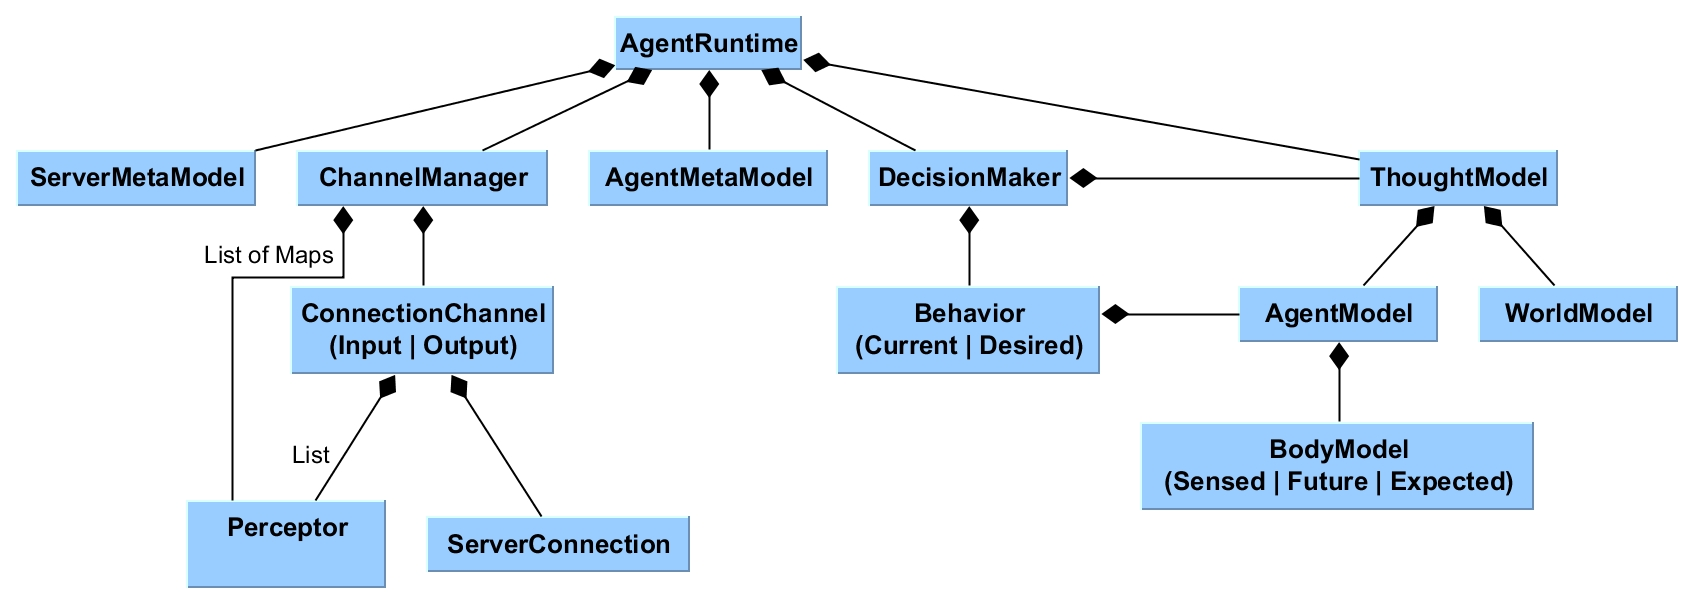
\includegraphics[width=\textwidth]{Grafiken/Magma/AgentRuntime_Structure}
	\caption{Magma Offenburg - Agent Runtime Architecture}
	\label{fig:Magma - Agent Runtime Struktur}
\end{figure}

In obiger Grafik kann man den groben Aufbau eines Magma Offenburg Agents erkennen. Die AgentRuntime ist der Java Prozess, welcher sich beim Server anmeldet und mit diesem kommuniziert. \\
\\
Für die Kommunikation ist der ChannelManager zuständig,  der die Verbindung zum Server vorhält, eingehende Daten verarbeitet (Parsen + update des Thoughtmodels) und ausgehende Daten serialisiert und an den Server weiterleitet.\\
\\
Das AgentMetaModel liefert Metainformationen über den simulierten Agent, wie verfügbare Gelenke und verfügbare Sensoren.\\
\\
Das ServerMetaModel enthält Informationen über den Server, wie aktuelle Versionsnummer, Dimensionen des Spielfelds und Namen der Landmarks.\\
\\
Hinter dem DecisionMaker verbirgt sich die komplette Logik des Agents. Der DecisionMaker entscheidet über die nächste auszuführende Behavior (Aktion). Grundlage für die Entscheidung ist das Thoughtmodel, in dem sowohl für den Spieler spezifische als auch alle Daten des Worldmodels enthalten sind.

\begin{figure}[H]
	\centering
	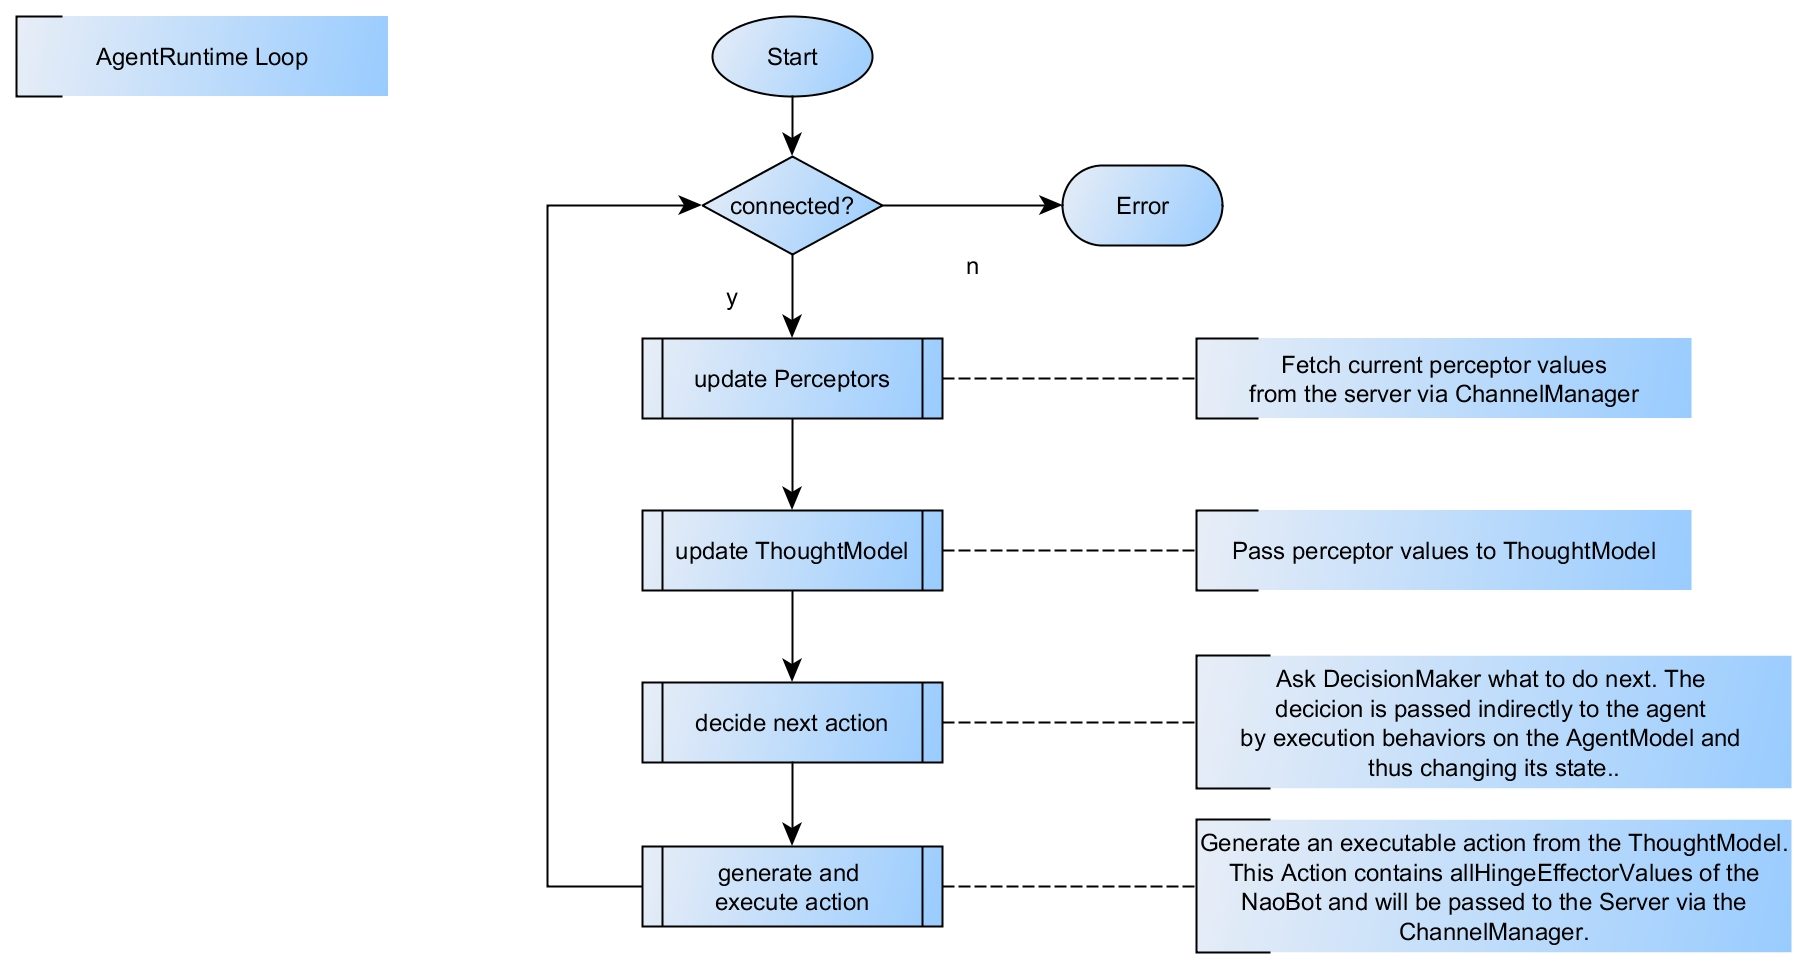
\includegraphics[width=\textwidth]{Grafiken/Magma/AgentRuntime_Loop}
	\caption{Magma Offenburg - Agent Runtime Loop}
	\label{fig:Magma - Agent Runtime Loop}
\end{figure}

Der Agent Runtime Loop beschreibt, was für jeden Zyklus im Agent passiert.\\
\\
Beim Eintreffen eines Pakets vom Server wird dessen Information geparsed und die erhaltenen Werte vom ChannelManager in die Liste der Perceptors (Daten über Gelenkwinkel und Sensoren) geschrieben.
Diese werden dann in jedem Zyklus in das Thoughtmodel übernommen.\\
\\
Im Anschluss fragt der Agent seinen DecisionMaker, welche Aktion er denn ausführen soll. Dieser überprüft anhand einer Reihe von Believes, welche Behavior denn ausgehend vom aktuellen Zustand des Thoughtmodels am sinnvollsten wäre und gibt diese zurück.\\
\\
Die für den nächsten Zyklus ausführbare Behavior wird nun wieder serialisiert und vom ChannelManager an der Server gesendet.\\
\\
Mit der Antwort des Servers beginnt ein neuer Zyklus.

\begin{figure}[H]
	\centering
	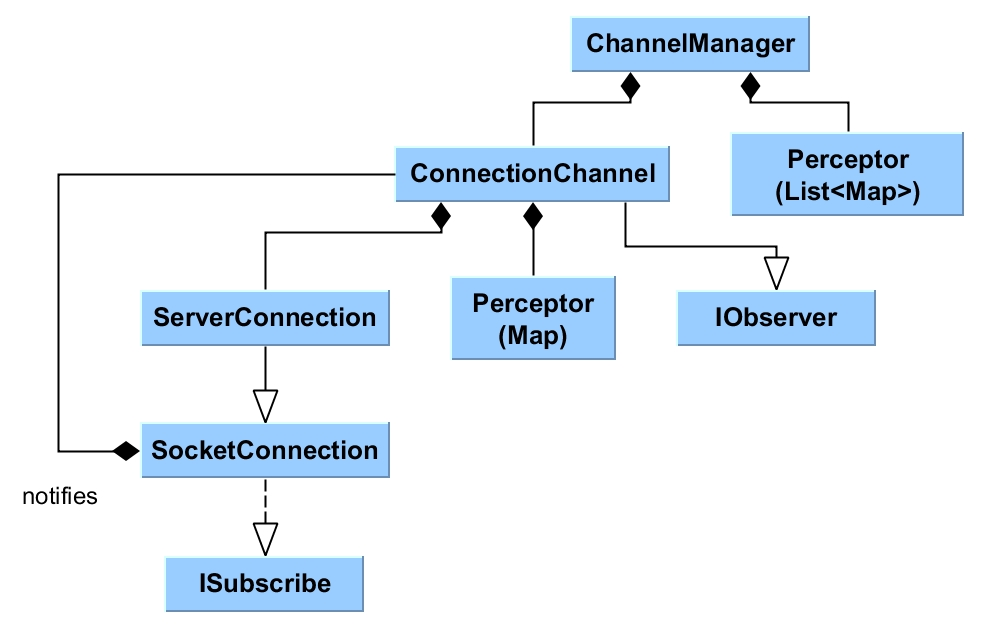
\includegraphics[width=\textwidth]{Grafiken/Magma/Observer_Structure}
	\caption{Magma Offenburg - Observer Structure}
	\label{fig:Magma - Observer Structure}
\end{figure}

Da der ChannelManager auf dem Observer Pattern basiert, möchte ich dieses noch kurz darlegen. Der ConnectionChannel meldet sich bei der SocketConnection als Observer an. Die SocketConnection hält die eigentliche Verbindung zum Server. Ist nun bei der Socket Connection ein Paket angekommen, informiert es alle seine Observer, also die ConnectionChannel, welche dann das Paket abholen, parsen und die enthaltene Information in den Perceptors abspeichern. Aus diesen werden sie dann vom Agent ausgelesen und in das Thoughtmodel übertragen. (siehe \autoref{fig:Magma - Agent Runtime Loop})

\subsubsection{Agent Startup Routine}
\label{subsec:Agent Startup Routine}
\textit{Verfasser: Stumpf}\\
\\
Welcher Agent mit welchen Eigenschaften gestartet werden soll ist über Kommandozeilenparameter konfigurierbar. Auf diese möchte ich im folgenden kurz eingehen:\\
\\
\texttt{--teamname="Robo1" --playerid=2 --server=192.168.56.101 --port=3100 --loglevel=severe --serverversion=68 --factory=NaoRF --decisionmaker=31 --homePosition=-15.0:0.0}
\begin{itemize}
\item \textbf{--teamname:} Der Name des Teams. Der rcssserver3d weist Agents vom gleichen Team der gleichen Seite zu.
\item \textbf{--playerid:} Die Spielernummer. Sollte unique sein.
\item \textbf{--server:} IP-Adresse des Servers.
\item \textbf{--port:} Port auf dem der rcssserver läuft. Standard ist 3100.
\item \textbf{--loglevel:} Das Loglevel des Agents. Nur console logging, nicht grafisch.
\item \textbf{--serverversion:} Version des Servers, entscheidet welche Serverkonfigurationsdatei verwendet wird.
\item \textbf{--factory:} Die Factory entscheidet, welches Agent-Modell verwendet wird. NaoRF ist ein von unserer Grupper erstelltes Modell, welches den Nao um einiege zusätzliche Bahaviors erweitert und Fehler in den maximalen Winkeln der Gelenke behebt.
\item \textbf{--decisionmaker:} Definiert den Decisionmaker für diesen Spieler. Zuweisung erfolgt nicht besonders elegant über einen Switch-Case in der Klasse ComponentFactory.java. Fall neue DecisionMaker angelegt und verwendet werden sollen müssen diese in der ComponentFactory hinzugefügt werden. Die 31 ist der von uns entwickelte Decisionmaker, der auf dem Strategy-Role-Modell (siehe \autoref{sse:KI-Gesamtübersicht}) basiert.
\item \textbf{--homePosition:} Dieser Parameter wurde von unserer Gruppe hinzugefügt. Damit lässt sich unabhängig von der Spielernummer eine HomePosition für den zu erstellenden Agent festlegen, von welcher aus dieser agiert.
\end{itemize}

Die Kommandozeilenparameter werden über die Klasse CommandlineParser.java eingelesen. Diese wurde wohl irgendwann einmal erweitert um obige Eingabemöglichkeit. Sollte der Commandline Parser irgendeinen der obigen --<param> Parameternamen nicht kennen, so wird er auf die alte Parser Version zurückfallen, die noch keine Namen für die Parameter kennt, sondern diese in einer bestimmten Reihenfolge erwartet. Das führt zu 100\% zu einem Fehler, sollte also beachtet werden.\\
\\
Unser KI-Konzept enthält einen Strategy Decider, der seine Entscheidungen anhand von Java-VM Parametern trifft. Sollte auf dem Strategy-Role-Konzept aufgebaut werden, bzw. dieses verwendet werden (z.B. DecisionMaker ID: 31), so müssen diese für eine korrekte Funktionalität gesetzt werden.\\
\\
Beispiel eines defensiven Spielers, der ebenso Freistoß, Einwurf und Ecke spielen darf(comma-separated values):\\
\\
\texttt{-DplayableRoles=Defense,CornerKick,FreeKick,ThrowIn}\\
\\
Verfügbare Primär-Rollen:
\begin{itemize}
\item Keeper
\item Defense
\item Middle
\item Attack
\end{itemize}

Verfügbare sekundäre Rollen:
\begin{itemize}
\item CornerKick
\item FreeKick
\item GoalKick
\item ThrowIn
\item KickOff
\end{itemize}

\subsubsection{Sammlung von Agent Startup Parametern}
\textit{Verfasser: Stumpf}\\
\\
Im Folgenden möchte ich meine Sammlung an Kommandozeile- und JVM-Parametern festhalten, die zum aktuellen Zeitpunkt unserer Magma Offenburg Weiterentwicklung verwendet werden können um:
\begin{itemize}
\item Ein Team zu erstellen
	\begin{itemize}
	\item \textbf{Keeper:}\\
\texttt{JVM: -DplayableRoles=Keeper,GoalKick\\
arg: --teamname="RoboFreunde" --playerid=2 --server=127.0.0.1 --		port=3100 --loglevel=severe --serverversion=68 --factory=NaoRF --		decisionmaker=31 --homePosition=-15.0:0.0}
	\item \textbf{Defense:}\\
\texttt{JVM: -DplayableRoles=Defense,CornerKick,FreeKick,ThrowIn}\\
\textbf{-Left:}\\
\texttt{arg: --teamname="RoboFreunde" --playerid=2 --server=127.0.0.1 --port=3100 --loglevel=severe --serverversion=68 --factory=NaoRF --decisionmaker=31 --homePosition=-10.0:5.0}\\
\textbf{-Mid:}\\
\texttt{arg: --teamname="RoboFreunde" --playerid=6 --server=127.0.0.1 --port=3100 --loglevel=severe --serverversion=68 --factory=NaoRF --decisionmaker=31 --homePosition=-10.0:0.0}\\
\textbf{Right:}\\
\texttt{arg: --teamname="RoboFreunde" --playerid=3 --server=127.0.0.1 --port=3100 --loglevel=severe --serverversion=68 --factory=NaoRF --decisionmaker=31 --homePosition=-10.0:-5.0}
	\item \textbf{MidField:} NOTE: Es wird abgeraten den Mittelfeldspieler zu verwenden, da dieser zum aktuellen Zeitpunkt unzureichend funktioniert!\\
\texttt{JVM:-DplayableRoles=Middle,CornerKick,FreeKick,ThrowIn,KickOff}\\
\textbf{-Left:}\\
\texttt{arg: --teamname="RoboFreunde" --playerid=8 --server=127.0.0.1 --port=3100 --loglevel=severe --serverversion=68 --factory=NaoRF --decisionmaker=31 --homePosition=-7.0:-4.0}\\
\textbf{-Mid:}\\
\texttt{arg: --teamname="RoboFreunde" --playerid=9 --server=127.0.0.1 --port=3100 --loglevel=severe --serverversion=68 --factory=NaoRF --decisionmaker=31 --homePosition=-7.0:0.0}\\
\textbf{Right:}\\
\texttt{arg: --teamname="RoboFreunde" --playerid=10 --server=127.0.0.1 --port=3100 --loglevel=severe --serverversion=68 --factory=NaoRF --decisionmaker=31 --homePosition=-7.0:4.0}
	\item \textbf{Attack:}\\
\texttt{JVM: -DplayableRoles=Attack,CornerKick,FreeKick,ThrowIn,KickOff}\\
\textbf{-Left:}\\
\texttt{arg: --teamname="RoboFreunde" --playerid=4 --server=127.0.0.1 --port=3100 --loglevel=severe --serverversion=68 --factory=NaoRF --decisionmaker=31 --homePosition=-4.0:2.5}\\
\textbf{-Mid:}\\
\texttt{arg: --teamname="RoboFreunde" --playerid=7 --server=127.0.0.1 --port=3100 --loglevel=severe --serverversion=68 --factory=NaoRF --decisionmaker=31 --homePosition=-2.0:0.0}\\
\textbf{-Right:}\\
\texttt{arg: --teamname="RoboFreunde" --playerid=5 --server=127.0.0.1 --port=3100 --loglevel=severe --serverversion=68 --factory=NaoRF --decisionmaker=31 --homePosition=-3.0:-2.5}
	\end{itemize}
\item Challenges zu starten
	\begin{itemize}
	\item \textbf{Kicks to Goal Challenge:}\\
\texttt{arg: --teamname="RoboFreunde" --server=127.0.0.1 --playerid=2 --port=3100 --loglevel=severe --serverversion=68 --factory=NaoRF --decisionmaker=12 --homePosition=-2.0:0.0}
	\item \textbf{Time to Goal Challenge:}\\
\texttt{arg: --teamname="RoboFreunde" --server=127.0.0.1 --playerid=2 --port=3100 --loglevel=severe --serverversion=68 --factory=NaoRF --decisionmaker=14 --homePosition=-2.0:0.0}
	\end{itemize}
\item Metrik-Agents zu starten
	\begin{itemize}
	\item \textbf{Kick Evaluation:}\\
\texttt{arg: --teamname="RoboFreunde" --server=127.0.0.1 --playerid=2 --port=3100 --loglevel=severe --serverversion=68 --factory=NaoRF --decisionmaker=26 --homePosition=-2.0:0.0}
	\item \textbf{Run Evaluation:}\\
\texttt{arg: --teamname="RoboFreunde" --playerid=2 --server=127.0.0.1  --port=3100 --loglevel=severe --serverversion=68 --factory=NaoRF --decisionmaker=13}
	\item \textbf{Dribble Evaluation:}\\
\texttt{arg: --teamname="RoboFreunde" --playerid=2 --server=127.0.0.1  --port=3100 --loglevel=severe --serverversion=68 --factory=NaoRF --decisionmaker=23}
	\item \textbf{Manual Keyboard Bot:} NOTE: Dieser Bot lässt sich mit einem Gamepad steuern. Unterstützt wird der XBox-Controller. Gedacht ist es, damit einen Agent in gewünschte Spielposition zu bringen und seine Reaktion zu testen.\\
\texttt{arg: --teamname="RoboFreunde" --playerid=2 --server=127.0.0.1  --port=3100 --loglevel=severe --serverversion=68 --factory=NaoRF --decisionmaker=100}
	\end{itemize}
\end{itemize}

\subsubsection{Verschiedene NAO-Models}
\label{sec:nao-models}
\textit{Verfasser: Schramm}\\
\\
Der Simspark-Server kann verscheidene NAO-Modelle simulieren. Diese unterscheiden sich zum
Beispiel in der Länge der Extremitäten oder der Existenz von Zehen. Im Server-Verzeichnis
liegen eine Reihe von Ruby-Scene-Graph-Dateien, welche die geometrische Beschaffenheit der
verschiedenen Typen definieren. Konnektiert ein Bot auf den Server, so schickt dieser in seiner initialen Nachricht einen String mit, der auf das entsprechende Modell verweist.\\

Im Magma-Framework werden diese verschiedenen Modelle durch eigene AgentMetaModel[s]
abgebildet. Diese sind in eigenen Packages unter 'magma.robots' organisiert. Initial waren
im fünf verschiedene Modelle enthalten. ('nao', 'nao1', 'nao2', 'nao3' und 'naotoe')\\
Mit Hilfe des RunToPositionMetricBots (siehe: \ref{sse:Elem Bew:Laufen}) wurde das Modell 'nao', welches auf der Server-Datei: 'rsg/agent/nao/nao.rsg' basiert als bestes ausgewählt. Im Zuge der Laufoptimierung wurden sämtliche Parameter mit denen aus der Server-Konfiguration verglichen.
Aufgrund von Abweichungen wurde dann ein eigenes AgentMetaModel 'NaoRF' im Package
'robofreunde' erstellt, das diese behebt.\\
So wurden zum Beispiel die Translationsvektoren der Füße von 'new Vector3D(0, 0.03, -0.035)'
auf 'new Vector3D(0, 0.03, -0.04)' verlängert. (Entsprechend der 'setLocalPos'-Z-Komponente
'(def \$FootRelAnkle\_Z -0.04)' in 'data/rsg/agent/nao/naoleg.rsg')

Die Auswahl der AgentMetaModel[s] erfolgt durch die zugehörige ComponentFactory (siehe: 
\ref{subsec:Agent Startup Routine} -factory). 

\subsubsection{DecisionMaker, Believes, Behaviors} \label{sse:decisionmaker-belives-behaviors}
\textit{Verfasser: Stumpf}\\
\\
DecisionMaker, Believes un Behaviors sind in Magma Offenburg ein eng verwobenes Konstrukt. Der DecisionMaker hat die Aufgabe, die Entscheidung über die nächste auszuführende Aktion zu treffen. Das zu implementierende Interface ist IDecisionMaker und definiert zwei relevante Methoden:
\begin{itemize}
\item \texttt{boolean decide();} Wird aufgerufen, wenn der DecisionMaker anhand des aktuellen Thoughtmodels eine Entscheidung über die nächste Aktion treffen soll. Überschreibt currentBehavior.
\item \texttt{IBehavior getCurrentBehavior();} Gibt die aktuell auszuführende Aktion currentBehavior zurück.
\end{itemize}

Die konkrete Implementierung des DecisionMakers kennt die Instanz des Thoughtmodels und hat somit immer Zugriff auf alle aktuellen Informationen. Die konkrete Entscheidung der nächsten Aktion ist ausgelagert in die Believes, wie man an folgendem Codeausschnitt der Implementierung von \texttt{decide()} sehen kann.

\begin{lstlisting}[caption=Ausschnitt aus decide(), captionpos=b, label=lst:DecidionMaker - decide()]
.
.
.
void decide() {
	.
	.
	.
	IBehavior toExecute = null;

	// temperature cool down
	toExecute = temperatureCoolDown();
	if (toExecute != null) {
		return toExecute;
	}
	// what to do when the game is finished
	toExecute = gameEndedAction();
	if (toExecute != null) {
		return toExecute;
	}
	// beam to this players starting position if it is allowed
	toExecute = beamHome();
	if (toExecute != null) {
		return toExecute;
	}
	.
	.
	.
	currentBehavior = toExecute;
}
.
.
.
protected IBehavior temperatureCoolDown()
{
	IBelief tooHot = believes.get(IBeliefConstants.TEMPERATURE_HOT);
	if (tooHot.getTruthValue() > 0.7) {
		return behaviors.get(IBehaviorConstants.SHUT_OFF);
	}
	if (tooHot.getTruthValue() > 0.4) {
		return behaviors.get(IBehaviorConstants.MOVE_ZERO);
	}
	return null;
}
.
.
.
\end{lstlisting}

Wie man in obigem Codeausschnitt sehen kann, werden der Reihe nach, nach Prioritäten geordnet, verschiedene Believes abgefragt. Sollte eine der Believes zutreffen, oder über einem Schwellwert sein (siehe Methode \texttt{temperatureCoolDown()}), so wird die damit verknüpfte Behavior zurückgegeben. Eine Behavior ist Zusammengesetzt aus Movements, von denen jede eine Reihe von gewünschten Winkelpositionen verschiedener Gelenke enthält, sowie Informationen in wie vielen Cycles und mit welcher Geschwindigkeit diese erreicht werden. Eine Behavior definiert somit einen Bewegungsablauf.
Beispiele für Behaviors sind:
\begin{itemize}
\item Aufstehen
\item Laufen
\item Kicken
\item Sich ausschalten
\item Nichts tun
\item Ball fokussieren
\item usw.
\end{itemize}

Meist prüfen die Behaviors selbst noch einmal, ob das mit ihnen verknüpfte Belief auch zutrifft. Zum Beispiel wird der Kick nur ausgeführt, wenn der Ball auch Kickable ist (Siehe Belief BallKickable). Falls nicht wird entweder die NullBehavior zurückgegeben, also nichts getan oder ein Fehler geworfen.

\subsubsection{Thought- und Worldmodel}
\textit{Verfasser: Stumpf}\\
\\
Das Thoughtmodel steht für die Datenhaltung des Agents. Es definieren den Zustand, in dem sich der Agent und das aktuelle Spiel gerade befinden. Nicht alle Daten sind im Thoughtmodel selbst enthalten, es fungiert jedoch als Container für Worldmodel, Flagmodel und Agentmodel. Das Worldmodel ist hiervon das wichtigste, da es die meisten Informationen enthält. Die Kommunikation über das Say-Interface des Servers wird praktischerweise ausgenutzt, um das Worldmodel aller eigenen Agents möglichst konsistent zu halten. Die Spieler tauschen darüber Informationen wie die eigene Position aus, die dann mit dem Worldmodel der anderen Spieler abgeglichen wird.
Positionen im Worldmodel sind immer aus Sicht des eigenen Teams angegeben. Der Ursprung des Koordinatensystems ist der Mittelpunkt des Spielfeldes. Die eigene Hälfte liegt dann im negativen Bereich der X-Achse, die gegnerische im positiven. Vom eigenen Tor aus gesehen links entspricht positiven Werten auf der Y-Achse, rechts negativen.\\
\\
Im Folgenden einige Thoughtmodel spezifische Informationen, diese stehen immer in Bezug zum eigenen Agent:
\begin{itemize}
\item \texttt{getObstacles()} Hindernisse, die ich (eigener Agent) umgehen muss.
\item \texttt{getPlayersAtMe()} Alle Spieler, geordnet nach Abstand zu mir.
\item \texttt{getOpponentsAtMe()} Alle Gegner, geordnet nach Abstand zu mir.
\item \texttt{...}
\end{itemize}

Das Worldmodel enthält die meisten für das Spiel relevanten Informationen:
\begin{itemize}
\item \texttt{Ball getBall()} Das Ball Objekt enthält Informationen über den Ball (u.a. seine Position).
\item \texttt{Vector3D getOwn/OpponentGoalPosition()} Position des eigenen/gegnerischen Tors. 
\item \texttt{GameState getGameState()} Spielstatus als Enum.
\item \texttt{PlaySide getPlaySide()} Spielfeldseite als Enum.
\item \texttt{float getGameTime()} Spielzeit.
\item \texttt{int getGoalsWe/TheyScored()} Anzahl der eigenen/gegnerischen Tore.
\item \texttt{...}
\end{itemize}

\subsubsection{Server Kommunikation}
\label{sec:server-communication}
\textit{Verfasser: Schramm}\\
\\
Die Kommunikation mit dem Server erfolgt über das Simspark-Protokoll. Im Framework wird diese Schnittstelle durch die Klasse:\\ \texttt{'magma.util.connection.impl.ServerConnection'} abgebildet. In einer Schleife werden dort die Pakete vom Server entgegen genommen und über das Observer Pattern an die \texttt{AgentRuntime} weiter geleitet. Diese verteilt die Daten über die \texttt{Perception} an die entsprechenden \texttt{Perceptoren}. So werden die Daten an die \texttt{Sensoren} (z.B. einen Joint) weitergeleitet.\\
Um in die Gegenrichtung Informationen zu senden wird durch die \texttt{Effektoren} eine \texttt{Action} generiert. Eine solche enthält den spezifischen Bezeichner des Effektors und den umzusetzenden Wert (vgl. Abb. \ref{fig:networkjointanalysis}).\\
Somit ist die gesamte Logik der Datenkonvertierung in den \texttt{Sensoren} und \texttt{Effektoren} gekapselt. In höheren Ebenen können so die Gelenke direkt manipuliert werden und die entsprechenden Befehle werden im nächsten Zyklus automatisch im richtigen Format an den Server gesendet.\\

Um die Kommunikation mit dem Server analysieren zu können bietet das Framework die Möglichkeit, den gesamten Verkehr zu loggen. So kann auf zusätzliche externe Werzeuge, wie Wireshark verzichtet werden und alle kommunizierten Daten werden direkt in Dateien geschrieben. Dazu muss in der \texttt{magma.robots.nao.general.ComponentFactory} in der Methode \textit{createChannelManager} ein \textit{SimsparkLogfileWriterChannel} mit dem \textit{ChannelManager} verknüpft werden. Ein Beispiel:\\

\begin{lstlisting}[caption=Loggen der Kommunikation, captionpos=b, label=lst:com-log]
@Override
public IChannelManager createChannelManager(ChannelParameters info)
{
	IChannelManager channelManager = new ChannelManager();

	File filePercept = new File("log/perceptions.log");
	File fileAct = new File("log/actions.log");
	InputOutputChannel channel = new SimsparkLogfileWriterChannel(channelManager
		,info, filePercept, fileAct);

	channel.init(createAgentMetaModel());
	channelManager.addInputChannel(channel, true);
	channelManager.addOutputChannel(channel);
	return channelManager;
}
\end{lstlisting}

\section{KI-Konzept}
\textit{Verfasser: Wurth}\\
\\
Für die KI wurde ein Konzept entwickelt, dass sich einfach in die bereits existierende Architektur des verwendeten Frameworks integrieren ließ. Ziel war es, eine möglichst flexible und gleichzeitig einfache Architektur zu entwerfen. Das Ergebnis ist eine Schichten-Architektur, deren Teilkomponenten einfach verändert oder ausgetauscht werden können. Nebeneffekte auf andere Module sind durch die Architektur weitgehend ausgeschlossen. So war es beispielsweise problemlos möglich, verschiedene Herangehensweisen für die Implementierung von Rollen in das Gesamtsystem zu integrieren. Verschiedene Teammitglieder konnten also ihre selbst entwickelten Rollen schnell und einfach in das Gesamtsystem integrieren, ohne andere Komponenten anpassen zu müssen.

\subsection{Anforderungen}
\textit{Verfasser: Wurth}\\
\\
Das gewählte Framework und die Notwenigkeit einer Steuerung für eigenständige Roboter, stellt einige Anforderungen an die zu entwickelnde künstliche Intelligenz.\\
\\
Jeder Roboter ist als unabhängiges Individuum zu verstehen. Das hat die direkte Folge, dass Entscheidungen nicht von einer übergeordneten Instanz getroffen werden können; Jeder Roboter muss aufgrund der ihm zur Verfügung stehenden Informationen selbstständig Entscheidungen treffen. Das Fehlen einer zentralen Komponente erschwert es erheblich, ein aufeinander abgestimmtes Team-Spiel zu entwickeln. Dennoch gibt es für dieses Problem gute Ansätze. Die Anforderung, die sich zusammenfassend daraus ableiten lässt, ist eine Lösung mittels einer dezentralen Architektur für die KI.\\
\\
Eine weitere Anforderung ergibt sich aus der Wahl des Frameworks. Das Framework arbeitet weitgehend mit Polling, also einem kontinuierlichen Abfragen der nächsten Aktion. Es ist daher naheliegend, auch für die hier zu entwickelnde KI einen Ansatz mit Polling zu zu verfolgen.\\
\\
Neben den mehr oder weniger durch die äußeren Umstände vorgegebenen Anforderungen haben wir noch zwei weitere Anforderungen definiert. Roboter sollen ihre Rolle dynamisch wechseln, außerdem soll es zusätzlich die Möglichkeit geben, die aktuell verfolgte Spiel-Strategie nach Bedarf zu ändern.

\subsection{Komponenten}
\textit{Verfasser: Wurth}\\
\\
Das KI-Grundkonzept besteht aus insgesamt 4 Schichten. Jede Schicht kennt ausschließlich die darunterliegende Schicht. Die unterste Ebene definiert die grundlegende Bewegungen eines Roboters. Direkt darüber befinden sich Rollen. Rollen sind zum Beispiel \glqq Stürmer\grqq{} oder \glqq Torwart\grqq, aber auch Spezialrollen wie \glqq Anstoß\grqq{} oder \glqq Freistoß\grqq. Über den Rollen befindet sich die Strategie-Ebene. Auf höchster Ebene befindet sich der Strategie-Entscheider. Die einzelnen Ebenen werden nachfolgend detaillierter beleuchtet.

\subsubsection{Elementare Bewegungen}
\textit{Verfasser: Wurth}\\
\\
Elementare Bewegungen sind die Grundlage für alle höheren Schichten. Sie sind die unmittelbare Voraussetzung die darüber liegenden Rollen, weil sie von diesen direkt benutzt werden. Elementare Bewegungen sind zum Beispiel: \glqq Laufen\grqq, \glqq Aufstehen\grqq, \glqq Schießen\grqq, oder \glqq Dribbeln\grqq. Abgesehen vom \glqq Dribbeln\grqq{} waren alle Bewegungen bereits mehr oder weniger funktionsfähig im Framework vorhanden. Dennoch musste an einigen Stellen optimiert und angepasst werden. Kapitel \ref{se:Elementare Bewegungen} widmet sich diesem Problem.

\subsubsection{Rollen}\label{Rollen Konzept}
\textit{Verfasser: Wurth}\\
\\
Ein Verteidiger verfolgt andere Ziele als ein Torwart. Rollen definieren das grundlegende Verhalten, also die grundlegenden Ziele eines Roboters. Alle unsere Rollen sind Statemachines, die allerdings unterschiedlich umgesetzt wurden. Eine wichtige Frage ist, wo und wie die KI für Standard-Situationen, wie zum Beispiel den \glqq Anstoß\grqq, in der Architektur verankert werden soll. Eine naheliegende Lösung ist die Definition von Spezialrollen, die genau diese Standard-Situationen behandeln. Die Alternative wäre eine Erweiterung aller Standard-Rollen um die Algorithmik der Standard-Situationen. Einen wirklicher Mehrwert ergibt sich daraus aber nicht, denn der Algorithmus um einen Anstoß durchzuführen benötigt keine Routinen eines Stürmers. Umgekehrt gilt das Selbe. Die Entscheidung fiel also auf die Definition von Spezialrollen, die genau diese Standard-Situationen umsetzen. Ein Roboter, dessen Rolle normalerweise Stürmer ist, wechselt bei Bedarf einfach seine Rolle in \glqq Anstoß\grqq{} und im Anschluss wieder zurück.

\begin{figure}[H]
	\centering
	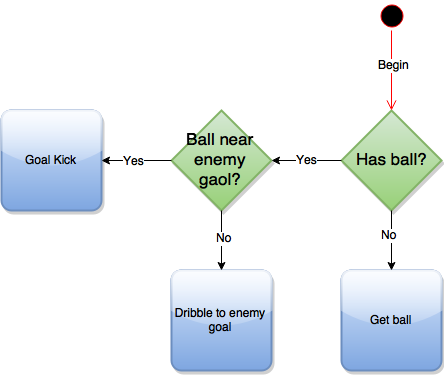
\includegraphics[width=0.7\textwidth]{Grafiken/KI/simple_Player}
	\caption{Beispiel Rolle: Einfacher Torwart}
	\label{Simple keeper}
\end{figure}

Abbildung \ref{Simple keeper} zeigt Beispielhaft den Entscheidungsbaum eines einfachen Torwarts.

\subsubsection{Strategien}
\label{StrategienLabel}
\textit{Verfasser: Wurth}\\
\\
Rollen sollen nicht selbst entscheiden, ob und in welche andere Rolle gewechselt wird. Das widerspräche der Schichtenarchitektur. Deshalb wurde die darüber liegende Strategieschicht eingeführt. Die Aufgabe dieser Schicht ist es, Rollen dynamisch zuzuordnen. Daher ist die Bezeichnung \glqq Strategie\grqq{} auch treffend; Eine Strategie steuert unter Anderem die Gesamtaufstellung des Teams. Damit lässt sich die allgemeine Spielweise des gesamten Teams steuern, mehr Verteidiger bedeutet eine defensive, mehr Angreifer eine aggressive Strategie. Eine Strategie benötigt einen Pool an Rollen, die sie \glqq verteilen\grqq{} darf. Dieser Pool legt indirekt die Spielweise eines Teams fest. Aufgabe jeder Strategie ist es dann, Rollen dynamisch nach Bedarf zu verteilen. Darunter fällt insbesondere auch die Vergabe der Spezialrollen.

\subsubsection{Strategie-Entscheider}
\label{StrategieEntscheiderLabel}
\textit{Verfasser: Wurth}\\
\\
In der Strategieebene können verschiedene Strategien für verschiedene Gesamtaufstellungen des Teams definiert werden. Im Laufe eines Spiels kann es sinnvoll sein, die Aufstellung an die Gegebenheiten und Anforderungen an das Spiel anzupassen. Dafür Wurde auf höchster Ebene ein Entscheidungsmechanismus etabliert. Die Aufgabe dieser Schicht ist es, je nach Bedarf eine passende Strategie auszuwählen. Dafür gibt es verschiedene Ansätze, zum Beispiel könnte eine passende Strategie je nach aktuellem Spielstand ausgesucht werden. Beispiel: 
\begin{itemize}
\item Mannschaft liegt vorne: Defensive Strategie
\item Unentschieden: Aggresive Strategie
\item Mannschaft liegt hinten: Aggressive Strategie
\item Mannschaft liegt hinten und Zeit läuft bald aus: Risiko Strategie
\end{itemize}

\begin{figure}[H]
	\centering
	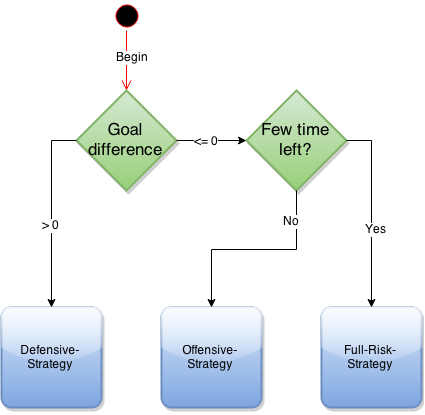
\includegraphics[width=0.7\textwidth]{Grafiken/KI/SimpleStrategyDecider}
	\caption{Einfacher Strategie Entscheider}
	\label{Einfacher Strategie Entscheider}
\end{figure}

Abbildung \ref{Einfacher Strategie Entscheider} zeigt den Enscheidungsbaum eines sehr einfachen Entscheidungsmeachanismus für Strategien.

\pagebreak

\subsection{Gesamtübersicht}\label{sse:KI-Gesamtübersicht}
\textit{Verfasser: Wurth}\\
\\
\begin{figure}[H]
	\centering
	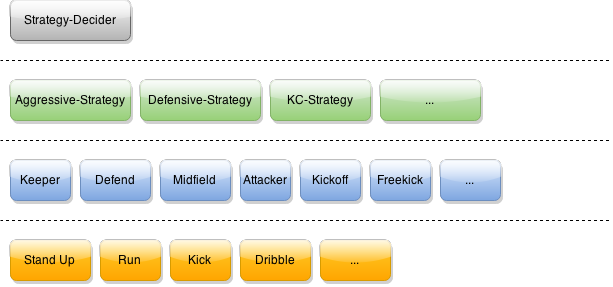
\includegraphics[width=1.0\textwidth]{Grafiken/KI/Ki-Concept}
	\caption{Gesamtkonzept KI}
	\label{Gesamtkonzept KI}
\end{figure}

Abbildung \ref{Gesamtkonzept KI} zeigt das Gesamtkonzept mit allen 4 Ebenen. Ganz unten befinden sich die elementaren Bewegungen. Rollen werden auf der Schicht darüber definiert. Sie greifen als einzige Schicht auf elementare Bewegungen direkt zu. Über den Rollen befindet sich die Strategie-Ebene. Jede Strategie hält einen Pool an Rollen vor und steuert damit die konkrete Aufstellung auf dem Spielfeld. Auf höchster Ebene befindet sich der Entscheidungsmechanismus, der Situationsabhängig eine passende Strategie aktiviert. 
\subsection{Alternative Ansätze}
\textit{Verfasser: Lohr}\\
\\
Es wurde recherchiert, wie eine KI am besten implementiert wird (Unter anderem in \cite{buckland2005programming}). Hierzu gibt es zwei Ansätze:
\begin{itemize}
 \item State-Driven Agent Design
 \item Goal-Driven Agent Design
\end{itemize}

\subsubsection{State-Driven Agent Design}
\textit{Verfasser: Lohr}\\
\\
Das State-Driven Agent Design basiert auf Zustandsautomaten, wie sie auch in UML definiert wurden. Ein Zustandsautomat setzt sich zusammen auf verschiedenen Zuständen (States), davon genau ein Startzustand und min. ein Endzustand. Die Übergänge (Transitions) von einem Zustand in einen anderen werden durch Ereignisse (Events) ausgelöst.

\begin{figure}[ht]
	\centering
  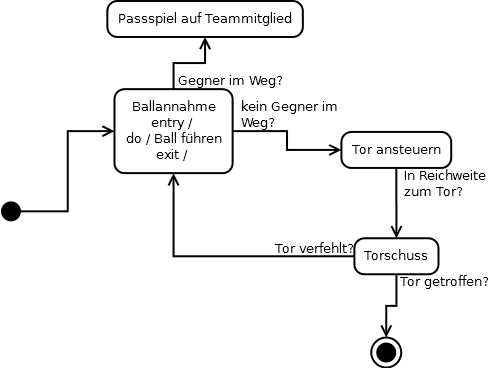
\includegraphics[width=0.7\textwidth]{Grafiken/KI/Bsp-Zustandsdiagramm.png}
	\caption{Ein stark vereinfachter Zustandsautomat}
	\label{fig1}
\end{figure}

Es gibt mehrere Möglichkeiten einen Zustandsautomaten zu implementieren. Es gibt unter anderem verschiedene Bibliotheken, die das implementieren eines Zustandsautomaten erleichtern. Unter anderem für C++: Boost.MSM (Meta State Machine), Boost.Statechart und Qt Statemachine Framework (aus dem Qt Framework). Für Java erschien die Tungsten FSM von Continuent am ausgereiftesten. Die Option ein auf Eclipse basierendes Tool namens Yakindu Statechart Tools\footnote{\url{http://statecharts.org/}} zu nutzen wurde verworfen, da nicht sicher war, wie sich das in den schon bestehenden Sourcecode einfügt.\par Die  Implementierung des Mittelfeldspieler mittels der Tungsten FSM wird auf der Seite \pageref{tungsten_fsm} im Abschnitt \ref{tungsten_fsm} erläutert.

\subsubsection{Goal-Driven Agent Design}
\textit{Verfasser: Lohr}\\
\\
Das Goal-Driven Agent Design wird in \cite[S. 379 ff.]{buckland2005programming} beschrieben. Es besteht aus Zielen, die entweder weitere Unterziele beinhalten können, oder sie sind selber ein atomarer Bestandteil, und haben keine weiteren Unterziele mehr. (vgl. Kompositionsmuster \ref{fig2} aus \cite{gamma1994design}) Ob ein Ziel erreicht wurde, wird dadurch bestimmt, ob gewisse Unterziele erreicht wurden oder nicht. Schlägt ein Ziel fehl kann es neu ausgeführt werden.

\begin{figure}[ht]
	\centering
  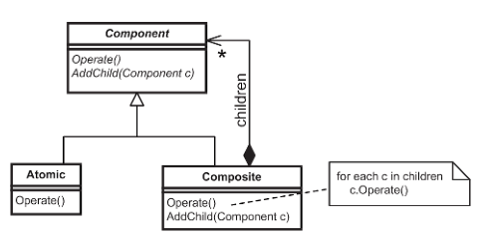
\includegraphics[width=0.7\textwidth]{Grafiken/KI/goal-driven.png}
	\caption{Das Kompositionsmuster. Grafik entstammt \cite[S. 383]{buckland2005programming}}
	\label{fig2}
\end{figure}

\subsection{KI-Architektur}
\textit{Verfasser: Weber}\\
\\
\begin{figure}[ht]
	\centering
  	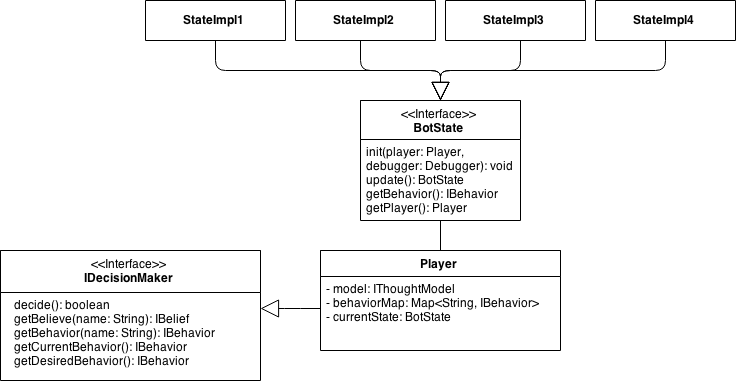
\includegraphics[width=1.0\textwidth]{Grafiken/KI/ki-architecture.png}
	\caption{Die KI-Architektur dargestellt in UML}
	\label{ki-architecture}
\end{figure}

Damit das entwickeln unterschiedlicher Komponenten sowie die Kommunikation mit dem Roboter reibungslos stattfinden kann, ist eine einheitliche Architektur sowie Schnittstelle zu dem benutzten Framework notwendig. Als Schnittstelle wurden die von Magma-Offenburg bereitgestellten \lstinline$Interface$s benutzt. Die erstellte Architektur ist der Abbildung \ref{ki-architecture} zu entnehmen, sie besteht aus zwei Hauptkomponenten, welche folgend erkl"art werden.

\paragraph{Player}
Diese Klasse implementiert die Magma Offenburg Schnittstelle und ist f"ur die Ausf"uhrung des aktuellen \lstinline$BotStates$ zust"andig.

\paragraph{BotState}
In diesem Interface wird die eigentliche Logik implementiert. Mit ihr wurde das State Design-Pattern umgesetzt.

\paragraph{Zusammenspiel der beiden Komponenten}
Die Rahmenklasse \lstinline$Player$, kennt wie bereits gesagt nur die aktuelle \lstinline$BotState$-Klasse. Der Aufruf zum aktualisieren der Logik wird "uber die \lstinline$update$ Methode an den \lstinline$BotState$ weitergereicht. Sollte dieser entscheiden dass ein "Ubergang zu einem anderen \lstinline$BotState$ notwendig ist, wird die Referenz auf diesen als R"uckgabeparameter geliefert. Damit ist die Rahmenklasse unabh"angig von der eigentlichen KI, sie ben"otigt lediglich die Referenz auf den Start \lstinline$BotState$. Die Rollen die als \lstinline$BotState$s definiert werden, sind f"ur ihre korrekte Ausf"uhrung selbst verantwortlich. Als Konsequenz bilden sich f"ur jede Rolle, kleinere Cluster von \lstinline$BotState$s die untereinander abh"angig sind. Durch dieses Vorgehen ist ebenfalls die Implementierung des Decorator Design-Pattern m"oglich, was wiederum f"ur die Strategien, sowie den Strategie-Entscheider ben"otigt wird.

\section{Elementare Bewegungen}\label{se:Elementare Bewegungen}
\textit{Verfasser: Stumpf}\\
\\
Im Laufe der Entwicklung hat sich herausgestellt, dass die in Magma Offenburg verfügbare Behaviors unzureichend waren für unsere Anforderungen.\\
\\
Es mangelte entweder an Funktionalität, oder an der Performance der Bewegungsabläufe. So war zum Beispiel weder Dribbeln, noch der Kick zu einer gegebenen Position implementiert und die Behaviors für Laufen und Kicken funktionierten denkbar schlecht.\\
\\
Es wurde demnach ein Teil des Teams mit der Implementierung und Optimierung benötigter Bewegungsabläufe beauftragt.

\subsection{Anforderungen}
\textit{Verfasser: Stumpf}\\
\\
Die Anforderungen an die neuen Behaviors kamen zum Teil aus dem KI-Team. So sind Dribbeln und ein Kick zu gegebener Position (KickToPosition) von den KI's vorausgesetzte Behaviors.\\
\\
Es fielen jedoch auch offensichtliche Mängel an einigen Behaviors auf, die es zu beheben galt. So war das Laufen von Magma Offenburg anfangs genau so wenig zu gebrauchen wie die implementierten Kicks.\\
\\
Mittels entwickelter Metriken und diese umsetzenden Metrik-Agents wurden die neuen und optimierten Behaviors mit den alten verglichen und getestet, um die Verbesserungen sichtbar zu machen. Sehr wichtig dafür war die Möglichkeit des grafischen Debugging mit RoboViz. (siehe \autoref{se:Grafisches Debugging})

\subsection{Laufen}\label{sse:Elem Bew:Laufen}
\textit{Verfasser: Schramm}\\
\\
Da die Laufleistungen der NAOs anfangs zu Wünschen übrig lies, wurde eine Optimierung vorgenommen. Zunächst wurde der RunToPositionMetricBot implementiert. Dieser läuft einen Parkour ab und misst die benötigte Zeit. Diese gilt als Metrik für die Laufoptimierung. Je kürzer die benötigte Zeit, desto besser die Lauffunktion.
Out-of-the-box erreichte der Bot innerhalb einer Halbzeit nicht einmal den zweiten Wegpunkt.
Danach erfolgte eine Verbesserung in drei Schritten:
\begin{itemize}
\item Laufgeschwindigkeit
\item Gelenkwinkelgeschwindigkeit
\item AgentMetaModel
\end{itemize}
Diese wurden iterativ abwechselnd ausgeführt, bis die Gesamtoptimierung in einem globalen Maximum angelangt war.

\subsubsection{Laufgeschwindigkeit}
Im ersten Schritt führte eine Reduktion der maximalen Laufgeschwindigkeit zu einer starken Abnahme von Stolperern. Die damit verbundene Einsparung an Aufstehungen führte somit trotz der langsameren Bewegung zu einer schneller Ankunft am Ziel.

\subsubsection{Gelenkwinkelgeschwindigkeit}
\label{subsubsec:joint-speed}
Im nächsten Schritt wurde mit der Konstante für die Gelenkwinkelgeschwindigkeit experimentiert (\textit{MAX\_JOINT\_SPEED} in  \texttt{magma.robots.nao.INaoConstants}). Eine Erhöhung dieses Werts führte zu einer stabileren und schnelleren Fortbewegung. Die Hoffnung, optimale Ergebnisse mit der serverseitigen Konstante zu erzielen, wurde leider enttäuscht.\\
Die ausgelesene Geschwindigkeit in den Config-Files von 6.14 ist in Grad pro Timeframe. Eine Umrechnung in rad/s, die der Server im Netzwerkprotokoll entgegen nimmt, ergibt 7.03. Dies entspricht dem Wert, der im Framework als Konstante definiert war und zu schlechten Ergebnissen führte.\\

Um mögliche Gründe hierfür zu finden wurde die Auswirkung der Konstante auf die tatsächlich erreichte Geschwindigkeit analysiert.
Als zu untersuchendes Gelenk wurde der Nacken gewählt, da sich dieser beliebig bewegen lässt ohne den Schwerpunkt des Naos zu verlagern und ihn somit umzuwerfen. So werden Seiteneffekte durch die Gesamtdynamik des Roboters vermieden. Andere Gelenke sind auf die selbe Weise implementiert und die Ergebnisse lassen sich übertragen.

Es wurde ein Test-Bot implementiert, der seinen Kopf so schnell dreht wie er kann. Dabei wurde die Netzwerkkommunikation mitgeschnitten und ausgelesen.
Bei einer Wahl von 7.03 rad/s als maximale Gelenkwinkelgeschwindigkeit im Framework fiel auf, dass diese nie an den Server kommuniziert wurde.

\begin{figure}[H]
	\centering
	\begin{tabularx}{\textwidth}{|X|X|X|}
		\hline
		Takt & Action & Perception\\
		\hline
		1 & (syn) & ... (HJ (n hj1) (ax -0.00)) ...\\
		\hline
        2 & (he1 -3.514)(syn) & ... (HJ (n hj1) (ax -4.03)) ...\\
        \hline
        3 & (syn) & ... (HJ (n hj1) (ax -8.05)) ...\\
		\hline
	\end{tabularx}
	\caption{Netzwerkauszug bei Kopfdrehung}
	\label{fig:networkjointanalysis}
\end{figure}

Trotz des Wunsches an das Framework eine Geschwindigkeit von 7.03 rad/s umzusetzen, gibt dieses nur die Hälfte, also 3.514 rad/s an den Server weiter.
Zu beachten gilt, dass der zurückgegebene Wert in Grad/Tick ist und somit dem Wunsch von 3.514 rad/s voll entspricht.

Dies ist auf die Implementierung der Motorrepräsentanten im Framework zurückzuführen.
Dort (\texttt{magma.agent.agentmodel.impl.Motor}) weist die 'getNextSpeed(float angle)' Methode folgenden code auf: \textit{return (angle - perceivedAngle) / 2.0f;}.\\
Der Motor erreicht durch die Halbierung des Winkels ein langsames Ausklingen an den Rändern der Bewegung. Nimmt man statt dessen den vollen Winkel erreicht der Nao auch die volle Geschwindigkeit von 7.03 rad/s, was leider durch ein Nachfedern an den Endpunkten begleitet wird. Werte von 80\% der Winkeldifferenz führen zu eine sauberen Bewegung.Leider kann der Nao mit diesen Einstellungen weder laufen, noch aufstehen. Die csv-Dateien der Bewegungen scheinen auf dieses Ausklingverhalten angewiesen, weshalb die ganze Analyse leider wenig Früchte trug und die Konfiguration zurückgesetzt wurde.

\subsubsection{AgentMetaModel}
Im letzten Schritt wurde das MetaModel des Agents im Framework mit dem des Servers verglichen und Unterschiede beseitigt. Auch dies hatte eine Erhöhung der Stabilität sowohl beim laufen, als auch beim Aufstehen zur Folge. Näheres dazu im Kapitel \ref{sec:nao-models}.
\subsection{Dribbeln}\label{sse:Elem Bew:Dribbeln}
\textit{Verfasser: Schramm}\\
\\
Für die Umsetzung verschiedener höher liegender Strategien ist es wichtig den NAO mit Ball an neue Positionen zu manövrieren. Eine Dribbelfunktion, die so etwas leisten könnte war jedoch im Framework nie vorhanden oder wurde entfernt. So war eine Konstante \textit{MOVE\_WITH\_BALL} zwar in \texttt{magma.agent.behavior.IBehaviorConstants} vorhanden, ihr wurde jedoch keine Implementierung zugewiesen.\\
Deshalb wurde ein eigenes Behavior zu diesem Zweck entwickelt\\
(\texttt{magma.robots.robofreunde.behavior.complex.DribbleWithBall}).

\subsubsection{Grundidee}
Da der Kick zum Entwicklungszeitpunkt der Dribbelfunktion nur sporadisch erfolgreich war, wurde als Grundlage das Laufen verwendet. Läuft der NAO gegen den Ball, so rollt dieser von ihm weg. Geschieht dies nun aus der richtigen Richtung, bewegen sich sowohl der Roboter als auch der Ball in die gewünschte Richtung. Aufgrund der geringeren Berührungsintensität am Ball, im Vergleich zum Kick, bleibt so auch die maximale Distanz zwischen diesem und dem NAO beim dribbeln kleiner.

\subsubsection{Positionierung}
Für die Positionierung zum Ball wird der relative Vektor von diesem zum Ziel berechnet und von dessen Position abgezogen. Die so berechnete Stelle liegt auf einer Linie mit dem Ball und dem Ziel. Erreicht der NAO diesen Ort, liegt der Ball genau zwischen ihm und dem gewünschten Ziel. In der Theorie schiebt der Roboter nun den Ball, während er sich auf das Ziel zu bewegt.

\subsubsection{Ball dribbeln}
Um zu verhindern, dass der NAO beim Versuch zu dribbeln den vor sich liegenden Ball als Hindernis erkennt, welchem er ausweichen soll, wurde ein neues Lauf-Behavoir (\texttt{magma.robots.robofreunde.behavior.complex.HulkToPosition}) vom bestehenden abgeleitet. Dieses ignoriert alle Hindernisse auf seinem Weg und bringt den NAO unsicher ans Ziel.

\subsubsection{Ausrichtung zum Ball}
Beim Bewegen zum gewünschten Ziel überprüft der NAO dabei ständig ob der Ball noch richtig liegt. Zu diesem Zweck wird ein Rechteck zwischen dem Ziel und der eigenen Position aufgespannt, dessen Breite kleiner ist als die des NAOs. Rollt der Ball nun über eine der Seitenlinien wird dies erkannt und eine Neupositionierung eingeleitet. Eine ungültige Seitenlinie wird im Debugger durch eine rote Färbung kenntlich gemacht, gültige sind grün.


\begin{lstlisting}[caption=Ausrichtung zum Ball, captionpos=b, label=lst:aligned-with-ball]
/**
 * Checks alignment with the ball via rectangle.
 * @param epsilon Allowed Distance from Ball to direct line.
 * @return True if the player is aligned with the ball.
 */
private boolean isAlignedWithBallReckt(double epsilon) {
    Vector3D leftPoint = getMyPosition().add(epsilon, new Vector3D(getAngleToPosition() + Math.toRadians(90), 0.0));
    Vector3D rightPoint = getMyPosition().add(epsilon, new Vector3D(getAngleToPosition() - Math.toRadians(90), 0.0));
    double leftAngleToBall = getBallPosition().subtract(leftPoint).getAlpha()
            - getMyPosition().subtract(leftPoint).getAlpha();
    double rightAngleToBall = getBallPosition().subtract(rightPoint).getAlpha()
            - getMyPosition().subtract(rightPoint).getAlpha();
    leftAngleToBall += leftAngleToBall < 0 ? 2* Math.PI : 0;
    rightAngleToBall += rightAngleToBall < 0 ? 2* Math.PI : 0;
    boolean isAlignedLeft = 0 < Math.toDegrees(leftAngleToBall) && Math.toDegrees(leftAngleToBall) < 90;
    boolean isAlignedRight = 270 < Math.toDegrees(rightAngleToBall) && Math.toDegrees(rightAngleToBall) < 360;
    if (!getDebugger().isHidden()) {
        getDebugger().drawLine(leftPoint
                , leftPoint.add(desiredBallPosition.subtract(getMyPosition()))
                , getValidationColor(isAlignedLeft));
        getDebugger().drawLine(rightPoint
                , rightPoint.add(desiredBallPosition.subtract(getMyPosition()))
                , getValidationColor(isAlignedRight));

    }
    return isAlignedLeft && isAlignedRight;
}
\end{lstlisting}

\subsubsection{Ausrichtung zum Ziel}
Da zwar der Ball im Rechteck liegen, der NAO aber verdreht zum Ziel stehen kann, wird auch diese Ausrichtung überprüft. Dabei der Winkel gemessen, der zwischen der aktuellen Ausrichtung des Bots und der Zielposition liegt. Ist dieser größer als ein zulässiger Maximalwert, wird eine Neupositionierung eingeleitet.\\
Befindet sich der NAO nahe am Ziel, ist eine größere Abweichung weniger schlimm, da schon kleine Änderungen im Ort große Auswirkungen auf den Winkel haben. Um diesem Umstand gerecht zu werden, wird der zulässige Maximalwert in Abhängigkeit zur Entfernung zum Ziel erhöht. Im Debugger werden die äußersten zulässigen Winkel durch Schenkelstücke dargestellt. Liegt das Ziel nicht innerhalb der Grenzen wechselt deren Farbe von Grün auf Rot.


\begin{lstlisting}[caption=Ausrichtung zum Ziel, captionpos=b, label=lst:facing-target]
/**
 * Checks whether the Nao is facing it's target.
 * @return True if the Nao is facing the target.
 */
private boolean isFacingTarget() {
    double validAngle = Math.toRadians(6.0) * getFuzzyMultiplier(desiredBallPosition);
    boolean isFacing = Math.abs(getAngleToPosition() - getPlayerAngle()) < validAngle;
    if (!getDebugger().isHidden()) {
        RoboVizColors color = getValidationColor(isFacing);
        getDebugger().drawLine(getMyPosition()
                , getMyPosition().add(new Vector3D(getPlayerAngle() - validAngle, 0.0)), color);
        getDebugger().drawLine(getMyPosition()
                , getMyPosition().add(new Vector3D(getPlayerAngle() + validAngle, 0.0)), color);
    }
    return isFacing;
}
\end{lstlisting}

\subsubsection{MetricBot}
Zur Bewertung des Optimierungsfortschritts wurde ein Decisionmaker implementiert, der einen gegebenen Parkour abdribbelt. Die benötigte Zeit gilt als zu minimierendes Kriterium. Im Laufe der Tests wurden so auch Schwächen einer Überprüfung der Ausrichtung zum Ball via Winkel aufgedeckt. Sie hatten die Implementierung der Funktion in ihrem aktuellen Zustand zur Folge.\\
In guten Versuchen liegt die benötigte Zeit für den Parkour mit einem Dribbeln des Balls nur circa ein Drittel höher als beim reinen Ablaufen ohne Ball.

\begin{figure}[H]
	\centering
	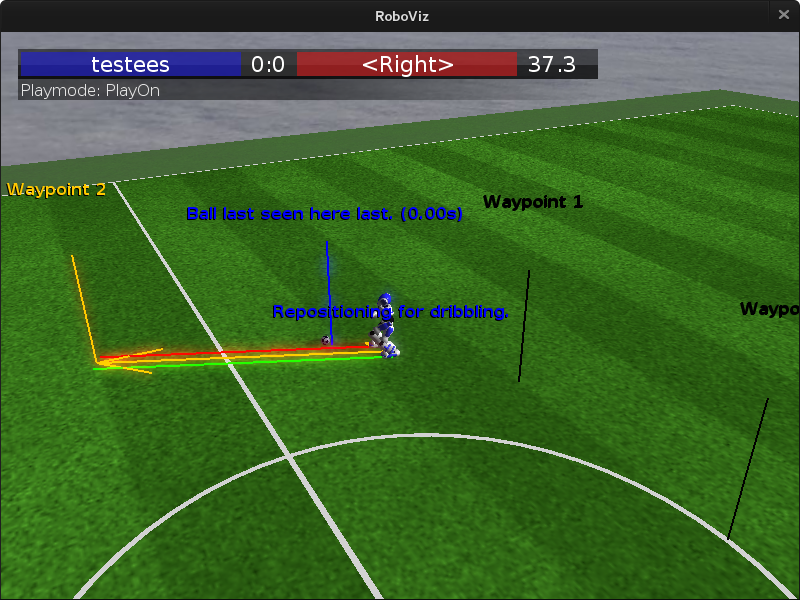
\includegraphics[width=\ScaleIfNeeded]{Grafiken/Dribble/DribbleRektReposition}
	\caption{Dribble Bot}
	\label{fig:dribblerekt}
\end{figure}
\subsection{Schie{\ss}en}\label{sse:Elem Bew:Schiessen}
\textit{Verfasser: Stumpf}\\
\\
Magma Offenburg bietet mehrere Implementierungen für den Ballschuss. Welche davon die geeignetste ist wurde zu Beginn anhand des Kriteriums \textit{\glqq Anschauen und Ausprobieren\grqq} festgestellt.\\
\\
Letztendlich haben wir uns dann für die KickStraight Behavior entschlossen. Diese hat eine recht umfangreiche Funktionalität. So wählt sie aus, welcher Fuß abhängig von der Spielerposition besser für den Kick geeignet ist. Zum anderen wird, abhängig davon ob ein Gegner in der Nähe ist oder nicht, entschieden ob ein schneller Kick oder der normale Kick ausgeführt werden soll.\\
\\
Die anderen erwähnenswerten Behavior sind: SlomoKick und KickStraight2. Es gibt noch eine Vielzahl an weiteren Kicks, diese sind aber entweder fehlerhaft (haben sich nicht vernünftig einbinden lassen), implementieren verschiedene Interfaces oder funktionieren schlecht bis gar nicht. Es liegt die Vermutung nahe, das viele der Kicks inzwischen deprecated, aber nicht als solche markiert sind.\\
\\
Da StraightKick nur den Bewegungsablauf eines geraden Kicks nach vorne definiert, wir aber einen Kick wollten der zu einer gegebenen Position kickt, wurde eine neue Behavior erstellt.\\
\\
\textbf{KickToPosition} bietet genau die gewünschte Funktionalität. Folgender Auszug zeit die Idee der Umsetzung.

\begin{lstlisting}[caption=KickToPosition, captionpos=b, label=lst:KickToPosition]
@Override
public IBehavior decideNextBasicBehavior() {
   updateInternalValues();
   myShootBehavior.setIntendedKickDirection(properKickPose.getAngle());
   // set relative pose to ball and angle to kick to
   myShootBehavior.setRelativeRunToPose(properKickPose.getX(), properKickPose.getY(), properKickPose.getAngle());
   myShootBehavior.setKickPower(kickPower);
   // is ball kickable calculates if the player is in a certain polygon, depending of the ball position
   if (myShootBehavior.isBallKickable() > 0) {
      return myShootBehavior;
   } else {
   // if the ball is not kickable reposition and run to proper kick pose
      RunToPosition runToPos = (RunToPosition) behaviors.get(IBehaviorConstants.RUN_TO_POSITION);
      runToPos.setPosition(properKickPose, 0, 0, 55, false);
      return runToPos;
   }
}
\end{lstlisting}

KickToPosition erbt von der Klasse ComplexBehavior, welche aus verschiedenen anderen Behaviors zusammengesetzt sein kann. Über die Methode \textit{decideNextBasicBehavior()} wird für den aktuellen Zyklus ausgewählt welche Behavior ausgeführt werden soll. Im Fall von KickToPosition sind die zwei zur Wahl stehenden Behaviors  RunToPosition (runToPos) um zu Laufen und ein über die Methode \texttt{void setUsedKick(String usedKick)} konfigurierbar Kick (myShootBehavior).\\
\\
In Zeile 3 werden für die Entscheidung benötigte Werte vorberechnet. Zeile 4 bis 7 aktualisiert diese für die intern verwendete Kick Behavior damit die Abfrage in Zeile 8 den erwünschten Wert zurückgibt.  \texttt{isBallKickable()} wird von einer Parentklasse implementiert und liefert zurück ob der Ball so liegt, dass man ihn kicken kann. Sollte die der Fall sein so werden wir schießen, wenn nicht wird über die RunToPosition Behavior eine Neupositionierung am Ball vorgenommen, so dass wir gut für einen Schuss zur Zielposition stehen.\\
\\
Im Verlauf der Entwicklung wurde letztendlich jedoch ersichtlich, dass der originale KickStraight aus folgenden Gründen nicht verwendbar ist.
\begin{itemize}
\item Fällt sehr oft hin
\item Kickt oft in den Boden
\item Nur ca. 60\% erfolgreiche Kicks
\item Reichweite unbefriedigend
\end{itemize}
Die Performance der Kicks musste also noch einmal grundlegend betrachtet und verglichen werden um anschließend eine Optimierung vornehmen zu können.
\subsubsection{Evaluierung, Metrik Bots}
\textit{Verfasser: Stumpf}\\
\\
Mit dem Ziel eine Vergleichsmöglichkeit für die Kicks zu schaffen habe ich folgende Punkte als Grundlage für eine Metrik definiert.

\begin{itemize}
\item Durchschnittliche Schussreichweite
\item Durchschnittliche Geschwindigkeit mit dem Ball vereint:
	\begin{itemize}
	\item Anteil erfolgreicher Schüsse (Schusssequenz kostet Zeit)
	\item Anteil der Schüsse ohne Hinfallen (Hinfallen kostet Zeit)
	\end{itemize}
\end{itemize}

Diese Metrik wurde umgesetzt im Agent KickEvaluation, der im Package\\ \texttt{magma.agent.decision.simple.robofreunde.role.evaluation.kick} zu finden ist. Dieser berechnet die oben definierten Werte anhand einem standardisierten Ablauf und verwendet das Roboviz Debugging um sie auszugeben.		

\begin{figure}[H]
	\centering
	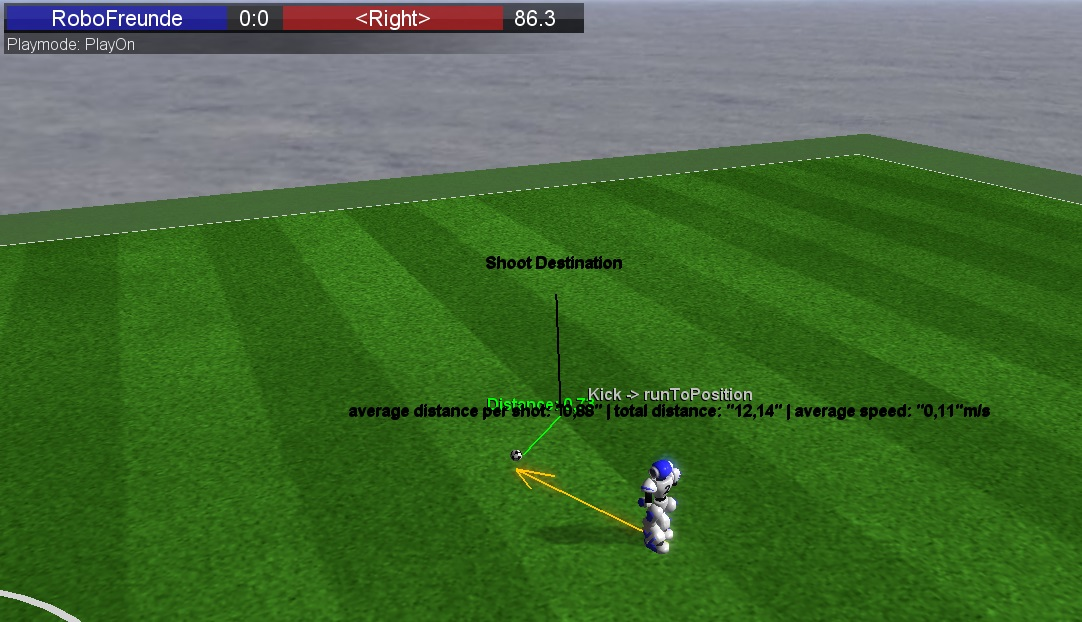
\includegraphics[width=\ScaleIfNeeded]{Grafiken/Kick/KickMetrikAgent}
	\caption{Ausgabe - Kick Metrik Agent}
	\label{KickMetrikAgent}
\end{figure}

Zusätzlich werden die Informationen noch auf der Konsole ausgegeben, um diese besser abspeichern und vergleichen zu können. Die Ausgabe wird mit jedem Schuss -- das hei{\ss}t der Ball hat sich bewegt -- aktualisiert.

\begin{lstlisting}[caption=Kick Metrik Konsolenausgabe, captionpos=b, label=lst:KickMetricConsoleOutput]
.
.
.
average distance per shot: "0,72" | total distance: "4,77" | average speed: "0,07"m/s
average distance per shot: "0,79" | total distance: "6,61" | average speed: "0,08"m/s
average distance per shot: "0,88" | total distance: "11,59" | average speed: "0,11"m/s
\end{lstlisting}

Die Evaluierung von SlomoKick, KickStraight und KickStraight2 des Magma Offenburg Frameworks ergab ohne Optimierung ähnliche Werte. Ich habe mich deshalb dazu entschieden, den ohnehin bereits verwendeten KickStraight zu optimieren.

\subsubsection{Optimierung}
\textit{Verfasser: Stumpf}\\
\\
Folgende Punkte konnten als Ursache der Probleme beim KickStraight festgestellt werden:
\begin{itemize}
\item Statisches Balancing!
\item Verwendung von nur einem Gelenk (Hüfte)
\item Kein Ausreizen der maximalen Winkel und Geschwindigkeit
\item Falsche, schlechte Werte (-> Boden-Kick)
\end{itemize}

Die nähere Analyse der Implementierung hat gezeigt, dass die Bewegungsphasen hart im Code definiert sind, was man in \autoref{lst:KickStraight-Movementphases} gut erkennen kann. In diesem Falle war das von Vorteil, da die Werte so sehr einfach manipuliert werden konnten.

\begin{lstlisting}[caption=KickStraight Bewegungsphasen, captionpos=b, label=lst:KickStraight-Movementphases]
.
.
.
kickRight.add(new MovementPhase("moveLegBackwards2", 20) //
	.add(INaoConstants.LHipPitch, 30, 1f) //
	.add(INaoConstants.LKneePitch, -20, 1f) //
	.add(INaoConstants.LFootPitch, 10, 0.5f) //
	.add(INaoConstants.RHipPitch, -5, 2f) //
	.add(INaoConstants.RKneePitch, -40, 2f) //
	.add(INaoConstants.RFootPitch, 20, 2f) //
	.add(INaoConstants.RHipRoll, 0, 1f) //
	.add(INaoConstants.RFootRoll, 16, 2f) //
	);
kickRight.add(new MovementPhase("kickRight", CYCLES_FOR_KICK) //
	.add(INaoConstants.LHipPitch, -50, 21f) // 
	.add(INaoConstants.LFootPitch, 33, 14f) // 
	.add(INaoConstants.LKneePitch, -16, 2f) // 
	.add(INaoConstants.RKneePitch, 6, 21f) // 
	);
.
.
.
\end{lstlisting}

Die größten Probleme bereitete das \textbf{statische Balancing}. Nach der Ausführung des Kicks erfolgten ursprünglich einige Bewegungsphasen, die den Roboter wieder in eine stabile Ausgangsposition bringen sollten. Da der Kick allerdings selten gleich verläuft -- der NAO ist nie in exakt der gleichen Ausgangslage -- hat dieses statische Balancing dazu geführt, dass der NAO meist das Gleichgewicht verloren hat und umgefallen ist.\\
\\
Diese Problem konnte behoben werden, indem die kompletten Bewegungsphasen für das Balancing entfernt wurden. Das funktioniert deshalb sehr gut, da direkt nach dem Kick die RunToPosition Behavior aufgerufen wird, um sich neu zu positionieren. Die RunToPosition balanciert sich hingegen viel besser und stabiler, vermutlich dynamisch.\\
\\
Des Weiteren führten \textbf{fehlerhafte Werte in den Bewegungsphasen} dazu, dass der NAO gerne in den Boden gekickt hat. Durch eine Anpassung der Gelenkwinkel sowie Winkelgeschwindigkeiten konnte dieses Problem deutlich verbessert werden.\\
\\
Durch \textbf{Erweiterung der Bewegungsabläufe um neue Gelenke} konnte sowohl die Geschwindigkeit, als auch die Stabilität des Schusses erhöht werden.\\
\\
Als Letztes wurde die \textbf{Gelenkwinkelgeschwindigkeit nicht ausgereizt}, zu der der NAO fähig ist. Durch die Erhöhung wurde durchschnittliche Reichweite des Schusses deutlich erhöht.\\
\\
Der optimierte Kick wurde als Behavior KickStraight3 abgespeichert und liegt im Package \texttt{magma.robots.robofreunde.behavior.basic;}\\
\\
Das Ergebnis der Optimierung kann man in folgender Tabelle sehen.

\begin{tabularx}{\textwidth}{|X|X|X|}
\hline
 & \textbf{KickStraight vorher} & \textbf{KickStraight3 Nachher}\\
\hline
\hline
 Distance & ca. 0.8m & ca. 2.6m\\
\hline 
 Speed & ca. 0.06m/s & ca. 0.2 m/s\\
\hline
 Fallen & 4/10 & 2/10\\
\hline
 Successful Kicks & 6/10 & 9/10\\
\hline
\end{tabularx}

\section{Rollen}
\textit{Verfasser: Wurth}\\
\\
Rollen legen fest, welches übergeordnete Ziel ein Roboter zu einem bestimmten Zeitpunkt verfolgt, aber vor Allem, wie dieses Ziel erreicht werden soll. Ziele wie Aufstehen nach einem Sturz, oder die eigene Position vor dem Ball korrigieren, sind untergeordnete Ziele, die vor allem in den elementaren Bewegungen verfolgt werden. Ein Stürmer, dessen finales Ziel es ist, ein Tor zu schießen, muss natürlich einige Schritte Vorarbeit zum Erreichen dieses Ziels leisten. Zum Beispiel muss er zuerst den Ball erobern. Die Algorithmik, die zum Erreichen eines solchen Ziels erforderlich ist, findet ihren Platz in den Rollen. Wie in Kapitel \ref{Rollen Konzept} bereits erwähnt, werden Rollen in zwei Kategorien unterteilt, nämlich Standard-Rollen und Spezial-Rollen.
\\

Unter Standardrollen fallen alle normalen Spielertypen wie Stürmer, Verteidiger oder Torwart. In diesem Projekt wurden insgesamt 4 Standardrollen implementiert, deren genauere Beschreibung in diesem Kapitel Platz findet. Die Implementierung der Standardrollen wurde von verschiedenen Team-Mitgliedern durchgeführt. Stürmer und Torwart wurden von einer Person, Verteidiger und Mittelfeldspieler auch von jeweils einer Person entwickelt. Die Herangehensweisen unterscheiden sich deshalb zwischen den Rollen stark.
\\

Spezialrollen wiederum kümmern sich um spezielle Situationen wie zum Beispiel den Anstoß oder den Kick-In.


\subsection{Standardrollen: Torwart und Stürmer}
\textit{Verfasser: Wurth}\\
\\
Die Rolle Torwart und die Rolle Stürmer wurden von einer Person entwickelt. Sie teilen sich deshalb ein gemeinsames Grundkonzept.

\subsubsection{Konzept}
\textit{Verfasser: Wurth}\\
\\
Wie alle anderen Rollen auch, sind die Rollen für Torwart und Stürmer State-Machines. Jede State-Machine beinhaltet mehrere States. Jeder State hat eine ganz bestimmte Aufgabe, zum Beispiel: Zu einer bestimmten Position laufen. Im Kern befindet sich innerhalb eines States nur die Parametrisierung einer konkreten elementaren Bewegung. Diese Bewegung kann dann mittels Poll von außen abgefragt werden.
\\

Der erste Ansatz zur Modellierung der State-Machine war klassisch; Jeder State hatte eine bestimmte Menge an Folgestates und konnte demzufolge ausschließlich in diese States übergehen. Nach und nach offenbarte sich aber die Problematik dieser Designentscheidung. Bei laufenden Tests viel auf, dass bestimmte Transitionen von einem in einen anderen State nicht bedacht wurden. Folglich musste die State-Machine überarbeitet werden. Das führte recht schnell zu einer anderen Herangehensweise; Jeder State hat jeden anderen State der State-Machine als potenziellen Nachfolger. Ein enormer Flexibilitätszuwachs zur ersten Variante. Jetzt konnte der Entscheidungsmechanismus zur Findung des nächsten States  zentral etabliert werden. 
\\

Dazu wurde für beide Rollen jeweils eine Basisklasse angelegt. Diese Klasse kümmert sich um das Vorhalten aller States der StateMachine. Außerdem findet in ihr die Methode Platz, die einen Folgestate auswählt. Diese Methode ist das Herzstück der Rolle, sie definiert was wann gemacht werden soll.
\\

\begin{lstlisting}[caption=Beispiel Basisklasse Stürmer, captionpos=b, label=Beispiel Basisklasse Stürmer]
public abstract class BaseAttackerCenter extends BaseState {
    private DribbleState dribbleState;
    private GoalKickState goalKickState;
    private GoToBallState goToBallState;
    private GoToPositionState goToPositionState;
    private PassState passState;

    public void bootstrap(DribbleState dribbleState, 
    					  GoalKickState goalKickState, 
    					  GoToBallState goToBallState, 
                          GoToPositionState goToPositionState, 
                          PassState passState) 
    {
        this.dribbleState = dribbleState;
        this.goalKickState = goalKickState;
        this.goToBallState = goToBallState;
        this.goToPositionState = goToPositionState;
        this.passState = passState;
    }

    public BaseState decideNextState() {
        ...
    }
}
\end{lstlisting}

Listing \ref{Beispiel Basisklasse Stürmer} zeigt den Aufbau einer Basisklasse für States am Beispiel des Stürmers. Sie bekommt in der Methode \lstinline$bootstrap()$ von außen alle States und hält sie dann vor. Außerdem befindet sich ab Zeile 21 die Methode \lstinline$decideNextState()$.
\\

Jeder konkrete State leitet von diesem Basis-State ab und erbt somit alle States der Statemachine sowie die Methode \lstinline$decideNextState()$.
\\

\begin{lstlisting}[caption=Beispiel eines konkreten States: GoToBallState, captionpos=b, label=Beispiel eines konkreten States: GoToBallState]
public class GoToBallState extends BaseAttackerCenter {
    IBehavior moveToBall;

    @Override
    public void init(Player player) {
        super.init(player);
        this.moveToBall = null;
    }

    @Override
    public BotState update() {
        BaseState nextState = decideNextState();

        if (nextState == this) {
            RunToPosition moveToBall = (RunToPosition) getPlayer().getBehavior(IBehaviorConstants.RUN_TO_POSITION);
            moveToBall.setPosition(calcProperRunToBallPose(), 0, 0, 75, false);
            this.moveToBall = moveToBall;
            return null;
        }
        return nextState;
    }

    @Override
    public IBehavior getBehavior() {
        return this.moveToBall;
    }
}
\end{lstlisting}

Listing \ref{Beispiel eines konkreten States: GoToBallState} zeigt beispielhaft den State, der für das Laufen zum Ball verantwortlich ist. Er hält eine sogenannte \lstinline$IBehavior$ vor, die am Ende für das Ausführen der Bewegung benötigt wird. Innerhalb des States findet also nicht die Ausführung der Bewegung statt, sondern nur deren Parametrisierung. In der \lstinline$update()$-Methode wird zunächst abgefragt, welcher State für die aktuelle Situation am besten ist (Zeile 12). Dazu wird die geerbte Methode \lstinline$decideNextState()$ aufgerufen. Nur wenn der zurückgegebene State er selbst ist, soll er seinen Code ausführen und die \lstinline$IBehavior$ bearbeiten (Zeilen 14 - 18). Wurde ein anderer State zurückgegeben, wird kein eigener Code ausgeführt und der neue State zurückgegeben (Zeile 20). Damit die \lstinline$IBehavior$ von außen abgerufen werden kann, wurde hierfür ein Getter erzeugt (Zeilen 23 - 26).
\pagebreak

\subsubsection{Standardrolle: Torwart}
\textit{Verfasser: Wurth}\\
\\
\begin{figure}[H]
	\centering
	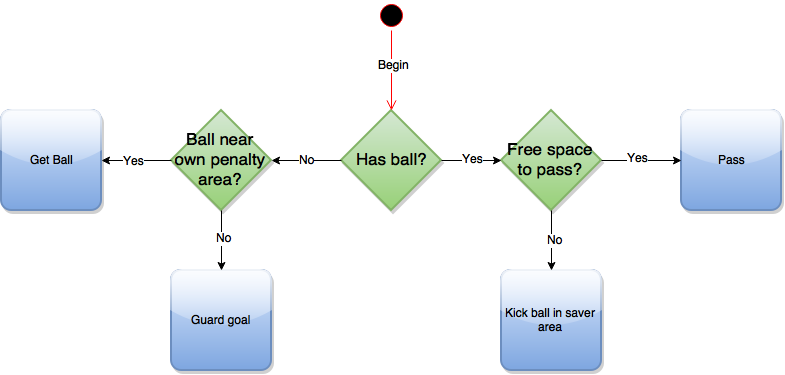
\includegraphics[width=\ScaleIfNeeded]{Grafiken/KI/Keeper}
	\caption{Torwart Entscheidungsbaum}
	\label{Torwart Entscheidungsbaum}
\end{figure}

Abbildung \ref{Torwart Entscheidungsbaum} zeigt den Entscheidungsbaum des Torwarts. Die Entscheidungsbäume von Torwart und Stürmer finden ihre direkte Umsetzung in der \lstinline$decideNextState()$ des Basis-States. Es war also sehr sinnvoll vor der Implementierung derartige Entscheidungsbäume zu entwerfen.
\\

\textbf{Der Entscheidungsbaum}
\\

Die Statemachine des Torwarts besteht aus insgesamt 4 States. Die erste Überprüfung ist, ob der Spieler den Ball besitzt. Besitzt er den Ball, will er ihn schnell wieder loswerden, schließlich ist er ein Torwart. Dazu sucht er im eigenen Team passende Passpartner. Ein passender Passpartner steht in einer passenden Entfernung und wird nicht von einem gegnerischen Spieler geblockt. Ist ein passender Spieler gefunden wird der Pass ausgeführt. Findet sich kein Spieler, soll der Ball in Richtung der Mittellinie geschossen werden, also möglichst weit weg vom eigenen Tor.
\\

Besitzt der Torwart den Ball nicht, kommt es auf die Entfernung des Ball an. Ist der Ball ein gutes Stück entfernt, soll in den State \lstinline$GuardGoalState$ gewechselt werden. Was dieser State genau macht wird später beschrieben. Kommt der Ball dem eigenen Tor zu nahe, soll der Torwart reagieren und auf den Ball zulaufen, um ihn zu erobern.
\pagebreak

\textbf{Der \lstinline$GuardGoalState$}
\\

Hat der Ball eine relativ große Entfernung zum Tor, soll sich der Torwart natürlich nicht vom eigenen Tor wegbewegen. Vielmehr sollte er eine geeignete Position vor dem Tor einnehmen. Ziel ist es, eine möglichst große Fläche des Tors zu \glqq verdecken\grqq, um Distanzschüsse zu verhindern oder zumindest zu erschweren. Dafür ist der \lstinline$GuardGoalState$ zuständig.
\\

\begin{figure}[H]
	\centering
	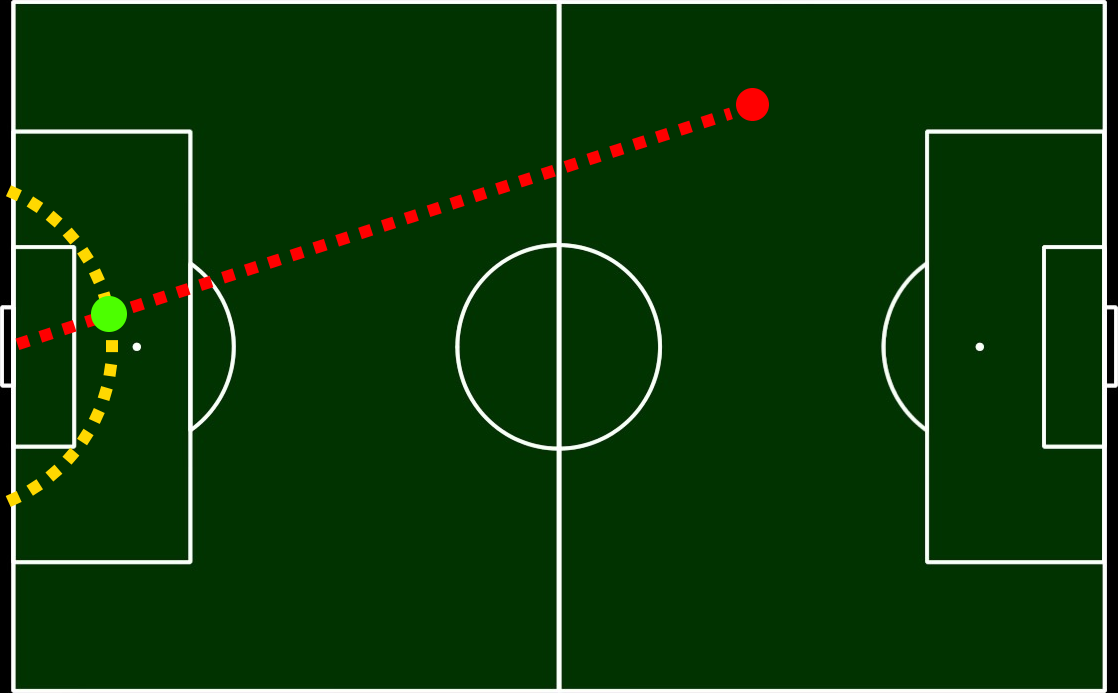
\includegraphics[width=\ScaleIfNeeded]{Grafiken/KI/guard_goal}
	\caption{Veranschaulichung des \lstinline$GuardGoalState$s}
	\label{Veranschaulichung des GuardGoalState}
\end{figure}

Abbildung \ref{Veranschaulichung des GuardGoalState} veranschaulicht die Berechnung der optimalen Position vor dem Tor anhand einer Grafik. Der gelbe Halbkreis definiert alle möglichen Positionen vor dem Tor, die der Torwart im \lstinline$GuardGoalState$ einnehmen kann. Die genaue Position hängt von der aktuellen Position des Balls ab. Dazu wird eine Gerade vom Ball in das Eigene Tor gelegt, der Schnittpunkt mit dem gelben Halbkreis entspricht der optimalen Position.
\\

\begin{lstlisting}[caption=Umsetzung des \lstinline$GuardGoalState$s, captionpos=b, label=Umsetzung des GuardGoalState]
public Vector3D getGoodGoalieDefendPosition() {  
	Vector3D ballPosition = thoughtModel.getWorldModel().getBall().getPosition();  
	Vector3D goalPosition = thoughtModel.getWorldModel().getOwnGoalPosition();    
	Vector3D direction = ballPosition.subtract(goalPosition);  
	direction = direction.normalize().scalarMultiply(2.0f);  
	return goalPosition.add(direction);  
}  

\end{lstlisting}

Listing \ref{Umsetzung des GuardGoalState} zeigt die Berechnung der korrekten Position im Code. Notwendig sind jeweils die Position des Balls und des eigenen Tors (Zeilen 2 und 3). Dann wird ein Richtungsvektor berechnet, der vom Tor in Richtung Ball zeigt (Zeile 4). Dieser wird zuerst normiert und dann auf die Länge 2 skaliert. Der Abstand 2 vom Tor hat sich als guter Wert herausgestellt (Zeile 5). Die gesuchte Position errechnet sich durch die Addition des Richtungsvektors auf die Torkoordinate (Zeile 6).
\\

\textbf{Energiesparmaßnahme}
\\

Der Torwart wird die meiste Zeit innerhalb des \lstinline$GuardGoalState$ bleiben. Bei jedem Poll wird eine neue Position anhand der Ball und Torposition berechnet, zu der er dann hinläuft. Bei Ball und Torkoordinate handelt es sich aber um circa Angaben, schließlich wird das Worldmodel anhand der Sensoren des Roboters kontinuierlich korrigiert. Dabei kommt es zu minimalen Schwankungen, die zu einer neu berechneten Laufposition führen. Somit kommt der Roboter quasi nie zum Stillstand, auch wenn er seiner berechneten Laufposition extrem nahe ist. Damit der Roboter stehen bleibt, wenn er hinreichend nahe an seiner Zielposition steht, wurde eine Energiesparmaßnahme eingeführt.
\\

\begin{lstlisting}[caption=Energiesparmaßnahme Torwart, captionpos=b, label= ESM Torwart]
if (nextState == this && (targetDistance > 0.2 || !angleCloseEnough(angleToBall))) {
	...
} 

\end{lstlisting}

Listing \ref{ESM Torwart} zeigt die Bedingungen für eine erneute Bewegnung. Nur, wenn die Zieldistanz einen hinreichend kleinen Wert überschreitet, oder der Winkel des Roboters zum Ball nicht gut genug ist, soll zur neuen Position gelaufen werden. Ursprünglich wurde nur die Distanz zum Ziel herangezogen, mit der Folge, dass der Roboter teilweise quer zum Ball stehen blieb. Damit verdeckt er aber weniger Fläche vom Tor, also wurde noch ein optimaler Winkel zum Ball miteinbezogen.

\pagebreak 

\subsubsection{Standardrolle: Stürmer}
\textit{Verfasser: Wurth}\\
\\
\textbf{Der Entscheidungsbaum}
\\

\begin{figure}[H]
	\centering
	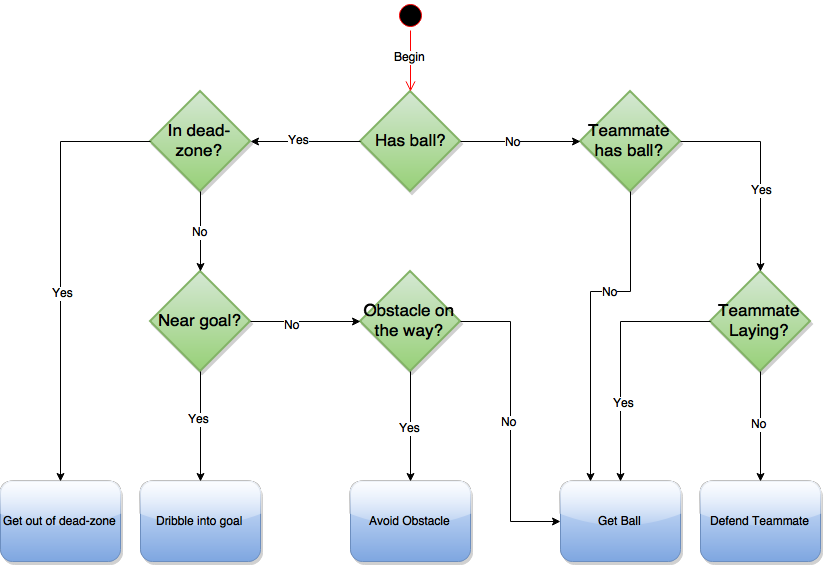
\includegraphics[width=\ScaleIfNeeded]{Grafiken/KI/attackerCenter_v2}
	\caption{Stürmer Entscheidungsbaum}
	\label{Stuermer Entscheidungsbaum}
\end{figure}

Abbildung \ref{Stuermer Entscheidungsbaum} zeigt den Entscheidungsbaum des Stürmers. Genau wie der Torwart, prüft auch der Stürmer als erstes, ob er in Ballbesitz ist. Wenn er den Ball nicht hat, prüft er, ob ein anderer Spieler den Ball besitzt. Sollte ein Teamkollege am Ball sein, soll er den Teamkollegen natürlich nicht stören oder ihm gar den Ball abnehmen. Er sollte in der Nähe des Teamkollegen bleiben und eingreifen, falls der Teamkollege den Ball verliert oder fällt. Besitzt der Stürmer den Ball, will er ihn natürlich ins gegnerische Tor bringen, in diesem Fall dribbeln. Dabei kann es passieren dass er in eine ungünstige Zone auf dem Spielfeld gerät, die er zuerst wieder verlassen muss (dazu später mehr). Ist der Stürmer mit seinem Ball unterwegs in Richtung gegnerisches Tor, ist es sehr wahrscheinlich, dass sich gegnerische Spieler in den Weg stellen. Er sollte also seine Laufbahn so anpassen, dass er Gegner im Optimalfall umläuft. Wie genau das geschieht wird auch später beschrieben. Ist der Stürmer dem gegnerischen Tor ausreichend nahe gekommen, soll er den Ball ohne Umwege hineindribbeln.
\\

\textbf{Warum schießt der Stürmer nicht?}
\\

Der Stürmer hat wider Erwarten keinen Zustand, in dem es zu einem Schuss kommen kann. In der ersten Version hat der Stürmer gepasst und auch Tore geschossen. Es hat sich jedoch bald herausgestellt, dass schießen sehr lange dauert. Der Roboter  muss sich vor jedem Schuss zuerst mühsam vor dem Ball positionieren. Außerdem war der Schuss bis kurz vor dem Endspiel, wenn er denn mal geklappt hat, eher kläglich. Das hätte dazu geführt, dass der Stürmer oft den Ball verliert. Deshalb wurde überall dort, wo normalerweise geschossen werden sollte, gedibbelt. Das Positionieren am Ball funktioniert beim Dribbeln sehr viel besser, dadurch geht weniger Zeit verloren. Der Verzicht auf Schüsse hat den Nachteil, dass das Passen komplett wegfiel, allerdings stellte sich das als ein eher kleines Übel heraus. Unser Stürmer passt nicht, unser Stürmer gewinnt, notfalls im Alleingang.
\\

\textbf{Gegnern ausweichen}
\\

Der Stürmer soll Gegnern auf dem Feld ausweichen und sie im Optimalfall umlaufen. Dazu muss er die Gegner natürlich erkennen und verstehen, dass sie sich in der Nähe seiner Laufline befinden und damit sehr wahrscheinlich ein Hindernis darstellen oder bald zu einem werden.

\begin{figure}[H]
	\centering
	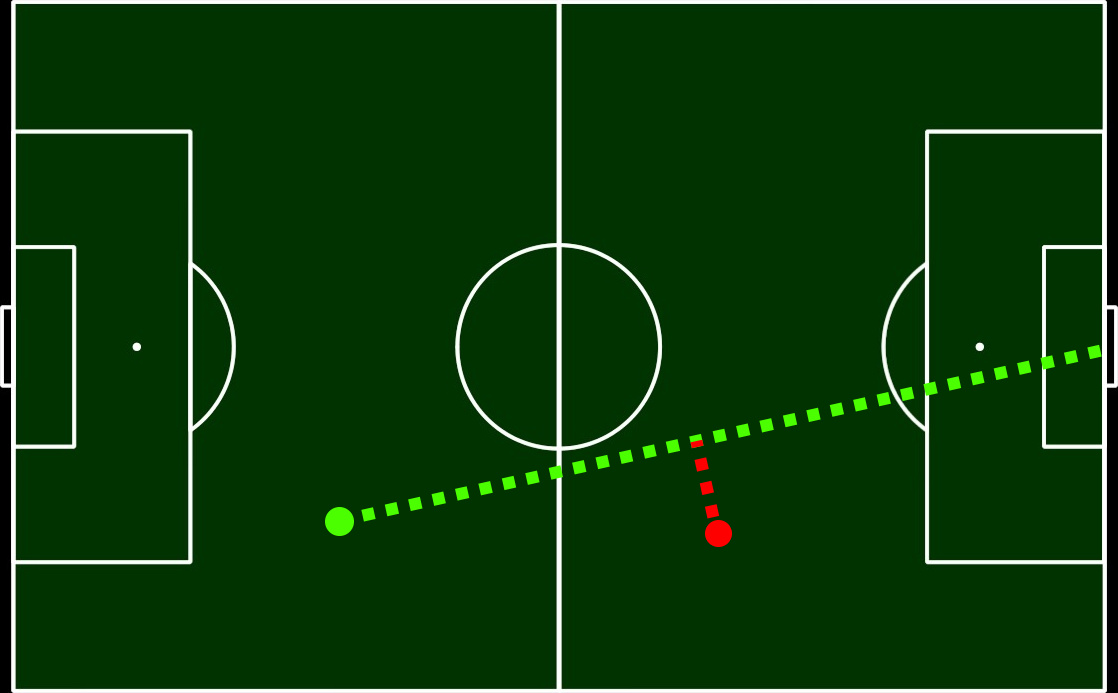
\includegraphics[width=0.8\textwidth]{Grafiken/KI/obstacle_2}
	\caption{Hindernis erkennen 1}
	\label{Hindernis erkennen 1}
\end{figure}

Abbildung \ref{Hindernis erkennen 1} zeigt diese Situation an einem Beispiel. Der gründe Punkt ist der Stürmer und seine Laufbahn wird mit der grün-gestrichelten Linie angedeutet. In der Nähe seiner Laufbahn befindet sich ein gegnerischer Spieler. Damit dieser als Hindernis erkannt werden kann, muss der Abstand aller gegnerischen Spieler  zur Linie geprüft werden. Unterschreitet der Abstand einen bestimmten Wert, wird der Gegner als potentielles Hindernis erkannt. Ziel ist es jetzt, den Abstand vom Gegner zur Lauflinie zu vergrößern.

\begin{figure}[H]
	\centering
	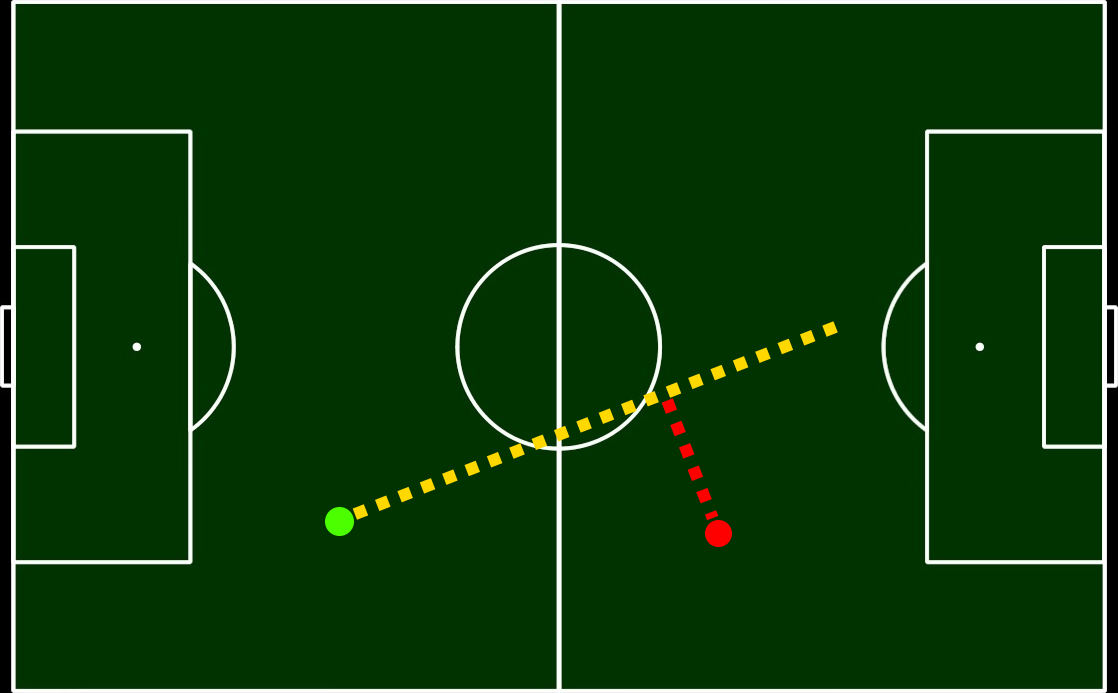
\includegraphics[width=0.8\textwidth]{Grafiken/KI/obstacle_3}
	\caption{Hindernis erkennen 2}
	\label{Hindernis erkennen 2}
\end{figure}

Abbildung \ref{Hindernis erkennen 2} verdeutlicht das Vorgehen. Um den Abstand zu erhöhen, muss die Zielposition geändert werden. In diesem Fall muss der Stürmer links am Gegner vorbei, also zu einer Position die weiter links liegt als die ursprüngliche. Ein rechts-seitiges Umlaufen des Gegners hätte 2 Nachteile. Erstens würde der Abstand vom Gegner zum Ball zuerst kleiner werden, bevor er wieder wächst. Das ist verschwendete Energie. Zweitens tendiert der Stürmer dann eher dazu den Seitenlinien zu nahe zu kommen. Die Vorgehensweise ist also auch eine natürliche Meidung der Spielfeldgrenzen, auch wenn sie nicht ganz ausreicht (dazu später mehr).
\\

Im fertigen Programm erkennt der Stürmer nur das Hindernis mit dem geringsten Abstand zu ihm. Das ist eine Vereinfachung, die aber trotzdem sehr gute Ergebnisse erzielt hat.
\\

\textbf{Deadzones}
\\

Bei einigen Tests viel auf, dass der State für das dribbeln nicht verhindert, dass gewisse ungünstige Zonen auf dem Spielfeld betreten werden. Ein Beispiel sind die natürlichen Grenzen auf dem Feld: Die Außenlinien.

\begin{figure}[H]
	\centering
	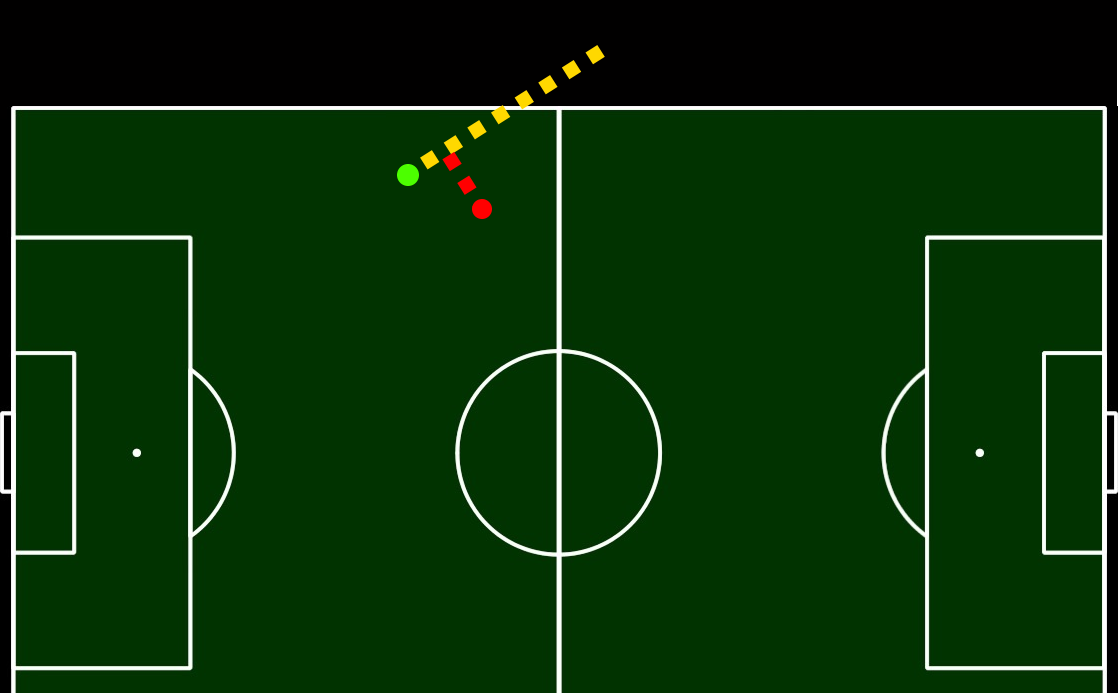
\includegraphics[width=0.8\textwidth]{Grafiken/KI/deadzone_1}
	\caption{Spielfeldgrenzen 1}
	\label{Spielfeldgrenzen 1}
\end{figure}

\begin{figure}[H]
	\centering
	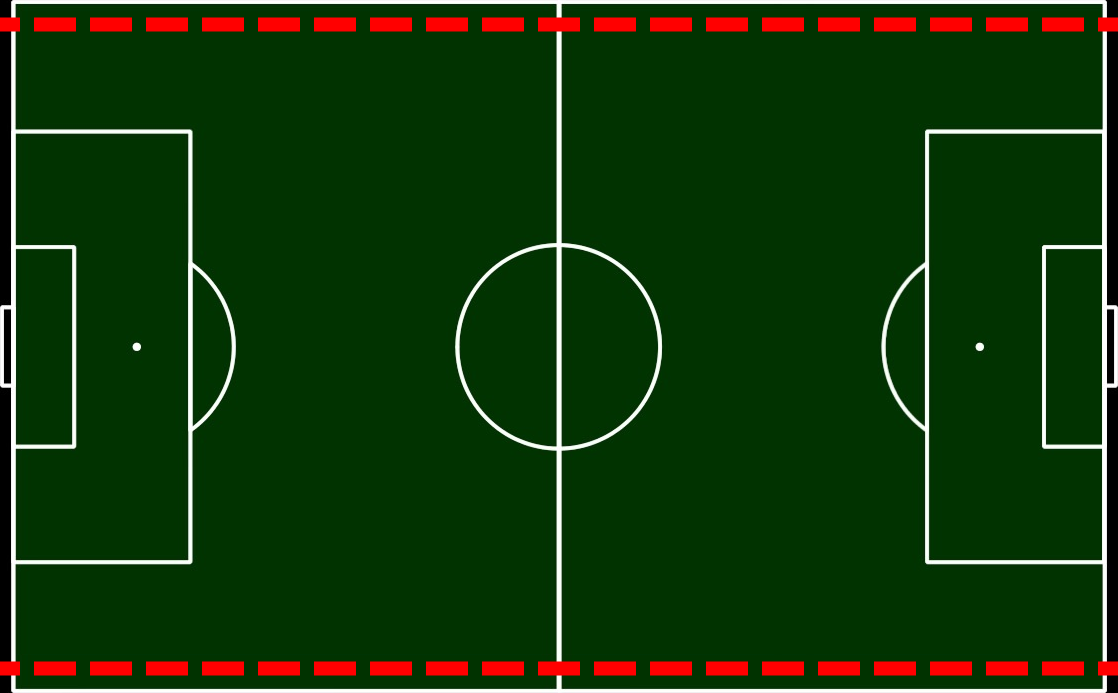
\includegraphics[width=0.8\textwidth]{Grafiken/KI/deadzone_2}
	\caption{Spielfeldgrenzen 2}
	\label{Spielfeldgrenzen 2}
\end{figure}

Abbildung \ref{Spielfeldgrenzen 1} zeigt, wie ein Stürmer beim Ausweichen das Spielfeld verlassen würde. Das muss natürlich verhindert werden. Die Lösung ist denkbar einfach, kurz vor den Außenlinien wurden Zonen etabliert (Abbildung \ref{Spielfeldgrenzen 2}), die nicht betreten werden dürfen, wenn der Stürmer den Ball besitzt.

\begin{figure}[H]
	\centering
	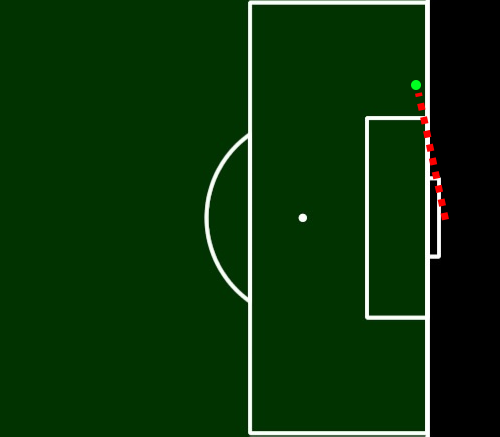
\includegraphics[width=0.7\textwidth]{Grafiken/KI/deadzone_5}
	\caption{Deadzone neben dem gegnerischen Tor 1}
	\label{Deadzone neben dem gegnerischen Tor 1}
\end{figure}

\begin{figure}[H]
	\centering
	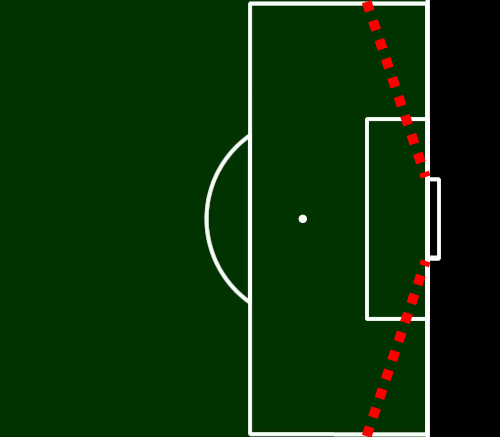
\includegraphics[width=0.7\textwidth]{Grafiken/KI/deadzone_3}
	\caption{Deadzone neben dem gegnerischen Tor 2}
	\label{Deadzone neben dem gegnerischen Tor 2}
\end{figure}

Abbildung \ref{Deadzone neben dem gegnerischen Tor 1} zeigt ein weiteres Problem. Ist der Stürmer dem gegnerischen Tor nahe genug, soll er direkt ins Tor dribbeln. Damit das auch wirklich zu einem Tor führt, muss die Position ein kleines Stück hinter die Torlinie gesetzt werden. Es könnte sonst dazu kommen, dass der Ball auf der Linie liegen bleibt. Das führt zu dem Problem, dass der Ball, der von einem gewissen Winkel zur Torlinie gespielt wird, noch vor dem Tor das Spielfeld verlässt. Damit das nicht passiert, macht es Sinn, auch hier Zonen zu definieren, die mit Ball nicht betreten werden sollen (Siehe Abbildung \ref{Deadzone neben dem gegnerischen Tor 2}).

\begin{figure}[H]
	\centering
	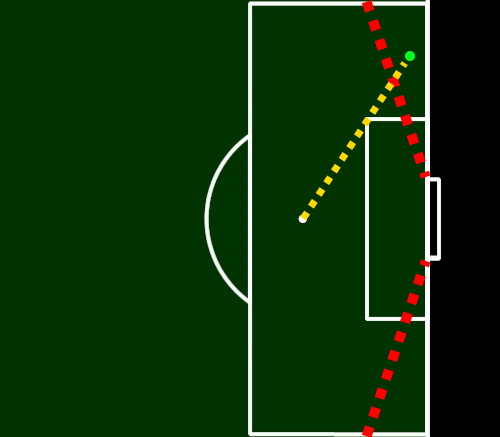
\includegraphics[width=0.7\textwidth]{Grafiken/KI/deadzone_6}
	\caption{Deadzone neben dem gegnerischen Tor 3}
	\label{Deadzone neben dem gegnerischen Tor 3}
\end{figure}

Es kann (und soll) aber dennoch vorkommen, dass sich ein Stürmer im Ballbesitz innerhalb einer Deadzone befindet. Nämlich dann, wenn er dort den Ball erobert. Bei den beiden Zonen in der Nähe der Aus-Linie korrigiert sich das Problem von alleine, die neue Laufposition befindet sich garantiert außerhalb. Bei den Zonen neben dem gegnerischen Tor, muss allerdings nachgeholfen werden. Die neue Laufposition befindet sich direkt vor dem Tor etwa in Höhe des Elfmeterpunktes (siehe Abbildung \ref{Deadzone neben dem gegnerischen Tor 3}). Das bedeutet natürlich nicht, dass er dieses neue Ziel tatsächlich erreicht. Sobald er die Deadzone verlässt ist sein Ziel erneut das gegnerische Tor.

\subsection{Standardrolle: Verteidiger}
\textit{Verfasser: Weber}\\
\\
\lstset{
    frameround=fttt,
    language=Java,
    numbers=left,
    breaklines=true,
    keywordstyle=\color{blue}\bfseries, 
    basicstyle=\ttfamily\color{black},
    numberstyle=\color{black}
    }

Der folgende Abschnitt beschreibt die Funktionsweise und den Prozess zur Erstellung der Rolle des Verteidigers.

\subsubsection{Vorgehensweise}
\textit{Verfasser: Weber}\\

\begin{figure}[H]
	\centering
	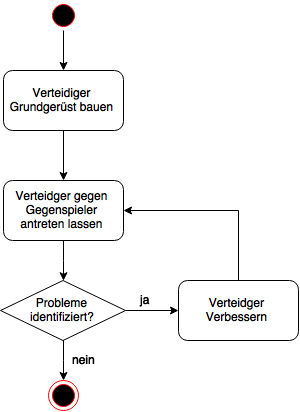
\includegraphics[width=0.5\textwidth]{Grafiken/KI/defender/vorgehensweise.png}
	\caption{Vorgehensweise zur Entwicklung des Verteidigers}
	\label{Vorgehensweise-Verteidigers}
\end{figure}
Der in Abbildung \ref{Vorgehensweise-Verteidigers} dargestellte Prozess ist der Anforderung geschuldet, zu einem m"oglichst fr"uhen Zeitpunkt bereits einen funktionierenden Spieler auf das Feld schicken zu k"onnen. Deswegen wurde ein iterativer Prozess gew"ahlt, zu Beginn wird ein einfaches Grundger"ust entwickelt. Dieses wird anschlie"senden zyklisch verbessert. Der Prozess kann verlassen werden, wenn keine Zeit mehr f"ur Verbesserungen vorhanden ist, oder keine weiteren Probleme identifiziert werden k"onnen.

\subsubsection{Use-Cases}
\textit{Verfasser: Weber}\\

\begin{figure}[H]
	\centering
	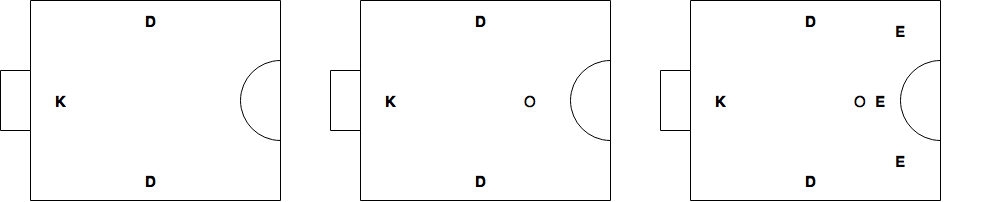
\includegraphics[width=\ScaleIfNeeded]{Grafiken/KI/defender/useCases.png}
	\caption{Die Use-Cases des Verteidigers}
	\label{Usecases-Verteidigers}
\end{figure}

F"ur den Verteidiger wurden die in Abbildung \ref{Usecases-Verteidigers} Use-Cases ermittelt. Die identifizierten Use-Cases hatten nicht den Anspruch alle m"oglichen F"alle abzubilden, sich aber auf einige wenige wichtige zu reduzieren. Bei der Erstellung der Use-Cases wurden mehrere idealisierende Annahme beachtet.

\begin{itemize}
\item Auf dem Spielfeld befinden sich nur Spieler der Rolle Verteidiger.
\item Der Verteidiger bewegt sich in jedenfall genau so schnell wie der Angreifer.
\item Der Verteidiger stellt ein Hindernis dar, welches umlaufen wird.
\end{itemize}

Generell wurde dem gegnerischen Spieler eine h"ohere Priorit"at zugeteilt als dem Ball. Falls der Ball nicht durch den gegnerischen Spieler in das Spielfeld getragen wird, versucht der Gegner den Ball f"ur sich zu erobern. Da die gegnerischen Spieler von dem Verteidiger gedeckt werden, sollten diese gleichzeitig bei dem Ball ankommen.

\paragraph{UseCase D1: Spielgeschehen auf anderer Spielh"alfte}
\label{UseCaseD1}
Weder der Ball noch Gegnerische Spieler befinden sich auf der eigenen Spielh"alfte.
\paragraph{UseCase D2: Ball in eigener Spielh"alfte}
\label{UseCaseD2}
Der Ball jedoch keine gegnerischen Spieler befinden sich auf der eigenen Spielh"alfte.
\paragraph{UseCase D3: Gegner (mit Ball) in eigener Spielh"alfte}
\label{UseCaseD3}
Gegnerische Spieler befinden sich auf dem Spielfeld. Dabei ist es unerheblich ob der Ball ebenfalls mit auf dem Spielfeld ist.

\subsubsection{Klassendiagramm}
\textit{Verfasser: Weber}\\
\begin{figure}[H]
	\centering
	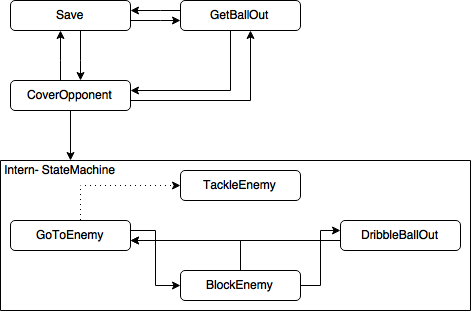
\includegraphics[width=0.8\textwidth]{Grafiken/KI/defender/defender.png}
	\caption{Vorgehensweise zur Entwicklung des Verteidigers}
	\label{Vorgehensweise-Verteidigers}
\end{figure}

Der Verteidiger wurde wie alle Rollen als State-Automat entworfen. Aus den Use-Cases wurden direkt 3 direkte Abbildungen entwickelt \lstinline{Save}, \lstinline{GetBallOut} und \lstinline{CoverOpponent}. Wobei die \lstinline{CoverOpponent}-Klasse noch eine internen State-Automat besitzt. Alle Klassen teilen sich die \lstinline{DefenseBaseState}-Klasse, die eine gewisse Basis-Funktionalit"at zur Verf"ugung stellt.

\paragraph{Save-State}
Der Save-State ist die Abbildung zum UseCase D1. In diesem State positioniert sich der Roboter nur auf seiner Home-Position und "uberwacht das akutelle Spiel auf Ver"anderungen.

\paragraph{GetBallOut-State}
Dient dazu den Ball aus der eigenen Spielfeldh"alfte zu entfernen. Urspr"unglich war dieser State eine exakte Abbildung des UseCases D2. Durch sp"atere Tests wurde die Transition zu diesem State erleichtert, sodass Situationen in denen der ``Ball als frei gilt'' ebenfalls eine Transition ausl"ost.\\
\\
Als frei wird der Ball bezeichnet (in der aktuellen Implementierung), wenn der n"achste Spieler am Ball vom gegnerischen Team und entweder zuweit entfernt oder umgefallen ist.

\paragraph{CoverOpponent-State}
In diesem State, werden ``freie gegnerische Spieler'' auf der eigenen Spielfeldh"alfte erkannt und der interne State-Automat ausgef"uhrt. Dieser bestimmt die exakten Aktionen des Roboters. Die \lstinline{CoverOpponent}-State Klasse ist lediglich daf"ur zust"andig den Gegner mit der h"ochsten Priorit"at zu finden, sollte ein solcher bestimmt worden sein, beginnt die Ausf"uhrung des internen State-Automaten beginnend mit der \lstinline{GoToEnemy}-Klasse.\\
\\
Als frei wird ein gegenerischer Spieler bezeichnet, wenn in seinem direkten Unfeld keine eigenen Spieler existieren, die ihn bereits decken. Sollten mehrere Spieler gefunden welche, dieses Kriterium erf"ullen, wird zuerst der Spieler mit dem Ball gedeckt, danach entscheidet die Distanz zum Tor.

\paragraph{GoToEnemy-State}
In erster Linie dient diese Klasse, wie der Name bereits verr"at, dazu eine Position zwischen dem Feind und dem Tor einzunehmen. Anschlie"send entscheidet die Klasse welche folge Zustand ausgef"uhrt werden soll. Der "Ubergang zu der \lstinline{TackleEnemy}-Klasse wurd im Verlauf der Entwicklung aus der Logik des Roboters entfernt.

\paragraph{TackleEnemy-State}
In dem urspr"unglichen Entwurf, sollte der Verteidiger mit einem gewichteten Zufall entscheiden ob er den Feind nach erreichen der Position, blockiert oder umwirft. Die Gewichtung konnte zum Konstruktionszeitpunkt bestimmt werden. Bei der aggressiven Strategie wurde zum Beispiel, die wahrscheinlichkeit f"ur ein Foul erh"oht. Jedoch wurde dieser State w"ahrend der Entwicklung verworfen, da das ``Tackeln'' sich als unstabil erwies.

\paragraph{BlockEnemy-State}
In dem ersten Entwicklungszyklus des Verteidigers, blockierte er nur den Weg des Verteidigers. Erst in dem Entwicklungsprozess wurde der letzte "Ubergang hinzugef"ugt und die Aufgaben der \lstinline{BlockEnemy} erweitert, sodass sie zus"atzlich darauf achtet ob der ``Gegner den Ball verliert''. Sollte dies der Fall sein, wird der "Ubergang zur \lstinline{DribbleBallOut} Klasse ausgef"uhrt.

\paragraph{DribbleBallOut-State}
Sollte der Roboter sich in diesem State befinden so bedeutet dies, wie bereits erl"autert, dass der Gegner den Ball verloren hat und er nun aus dem Spielfeld gebracht werden muss. Der State sucht nach Hindernissen, und versucht den Ball vor die Mittelfeldbegrenzung zudribbeln. Sollte dies erfolgreich verlaufen sein, schie"st er den Ball zu einem seinen Mitspielern.

\subsubsection{Wahl der Szenarien}
\textit{Verfasser: Weber}\\

Der Verteidiger wurde mit 3 Zyklen evaluiert.

\paragraph{Antritt gegen manuellen Bot}
Testen der "Uberg"ange gegen einen menschlich gesteuerten Roboter.

\paragraph{Antritt gegen SimpleBot}
In den ersten Runden wurde ein gr"osseres Problem entdeckt. Die erste Annahme, das ein Gegner stehen bleibt, war nicht haltbar. Das sich auch bei dem Testspiel mit Team KKB best"atigte. Deswegen wurde in diesem Zyklus die \lstinline{DribbleBallOut} Klasse zu dem internen State-Automat hinzugef"ugt. Bei den Tests wurde auch festgestellt, dass der State \lstinline{TackleEnemy} nicht die gew"unschte Leistung produzierte und wurde verworfen. Einige weitere Stellschrauben waren dar"uber hinaus, das Kriterium zur Erreichen der Position in der \lstinline{GoToEnemy} Klasse, die eigentliche Positions Bestimmung (unter Beruecksichtsnahme der distanz der beiden Roboter), sowie die Kriterien f"ur den "Ubergang von \lstinline{BlockEnemy} auf \lstinline{DribbleBallOut} State.

\paragraph{Antritt gegen St"urmer}
Verbesserungen in diesem Zyklus waren haupts"achlich das der "Ubergang von der \lstinline{CoverOpponent} zur \lstinline{GetBallOut} erleichter wurden. Ebenfalls wurde die \lstinline{DribbleBallOut}-Klasse erweitert, sodass sie nun das Ausweichen von mehreren Gegnern enthielt und den Pass zu eigenen Spielern. Als letzte Ma"snahme wurde der "Ubergang von der \lstinline{BlockEnemy} zur \lstinline{DribbleBallOut} erweitert.





\subsection{Standardrolle: Mittelfeld}
\textit{Verfasser: Lohr}\\
\\
\subsubsection{Tungsten FSM}
\label{tungsten_fsm}
\textit{Verfasser: Lohr}\\
\\
Es wurde das Tungsten FSM von Continuent für eine Beispielimplementierung herangezogen. Die Tungsten FSM besteht unter anderem aus
\begin{itemize}
 \item States
 \item Transitions
 \item Actions
 \item Guards
\end{itemize}
Die Funktionsweise wurde im Wiki (Robofreunde n. V.) unter Tungsten\_FSM festgehalten. Die grundlegenden Funktionen seien hier nochmal wiederholt:

\paragraph{States}
Zustände werden wie folgt definiert:
\begin{lstlisting}
State haveBall = new State("Habe_Ball", StateType.START);
State gotoGoalWithBall = new State("Laufe_zu_Tor", StateType.ACTIVE);
State shootBallToGoal = new State("Torschuss", StateType.END);
\end{lstlisting}
Es gibt drei Arten von Zuständen:
\begin{itemize}
 \item \underline{Start}: Jede Statemachine hat genau einen Startzustand. Nach dem Start der Machine geht diese automatisch in diesen Zustand
 \item \underline{End}: Jede Statemachine braucht min. einen Endzustand. Dieser terminiert die Statemachine
 \item \underline{Active}: Jeder Zustand, der weder Start- noch Endzustand ist
\end{itemize}

\paragraph{Transitions}
Ein Zustandsübergang wird dadurch definiert von welchen Zustand aus er in welchen Zustand wechselt und unter welchen Umständen (Guard) und welche Aktion (Action) er dabei ausführt. In dem nächsten Beispiel sieht man einen Übergang von Zustand 1 in Zustand 2, falls ein Event vom Typ MeinEvent auftritt. Dabei wird die Action NullAction ausgeführt:
\begin{lstlisting}
Transition t = new Transition("Zustand1_zu_Zustand2", new EventTypeGuard(MeinEvent.class),
                    zustand1, new NullAction(), zustand2);
\end{lstlisting}

\paragraph{StateTransitionMap}
Alle Zustände und Zustandsübergänge werden in einer Map gespeichert:
\begin{lstlisting}
StateTransitionMap map = new StateTransitionMap();
map.addState(zustand1);
map.addState(zustand2);
map.addTransition(t);
\end{lstlisting}

\paragraph{Action}
Eine Action wird beim Übergang in einen anderen Zustand oder beim Eintritt oder Austritt aus einem Zustand ausgeführt. Das Interface Action ist zu implementieren, und eine Methode \underline{doAction} muss definiert werden:
\begin{lstlisting}
public class NullAction implements Action{
        @Override
        public void doAction(Event message, Entity entity, Transition transition, int actionType) 
        throws TransitionRollbackException, TransitionFailureException, InterruptedException
        {
            // Hier kommt die Logik hin
        }
    }
\end{lstlisting}

\paragraph{Guard}
Ein Guard überprüft, ob ein Zustandsübergang genommen wird, oder nicht. Ein Guard muss das Interface Guard implementieren und die Methode \underline{accept} definieren:
\begin{lstlisting}
public class OwnGuard implements Guard
{
    @Override
    public boolean accept(Event message, Entity entity, State state)
    {
        // Hier kommt die Logik hin
    }   
}
\end{lstlisting}
Es gibt bereits einige vordefinierten Guards, wie z.B. EventTypeGuard, der nur positiv wird, wenn ein bestimmter Zustand geworfen wird.

\subsubsection{Mittelfeldspieler}
\textit{Verfasser: Lohr}\\
\\
Mit der Tungsten FSM wurde neben einem minimalen Bot auch ein Bot programmiert, der die Rolle ``Mittelfeldspieler'' einnehmen soll. Es wurden unter anderem folgende Use-Cases aufgestellt:

\begin{itemize}
 \item Eigene Mannschaft im Ballbesitz
 \begin{itemize}
  \item Solange die eigene Mannschaft im Ballbesitz ist, soll der Bot Abstand zum Ball halten
  \item Der Bot soll passiv bleiben, und versuchen das Vorankommen von gegnerischen Spieler zu verhindern
  \item Positionierung evtl. zwischen einem gegnerischen Spieler und dem ballbesitzendem eigenen Spieler um diesem einen, vom Gegner ungehinderten Lauf in Richtung Tor zu ermöglichen
 \end{itemize}
 
 \item Gegner im Ballbesitz
 \begin{itemize}
  \item Der Bot soll versuchen aktiv dem Gegner den Ball abzunehmen
  \item keine Behinderung von eigenen Mitspielern
 \end{itemize}
 
 \item Eigener Spieler im Ballbesitz
 \begin{itemize}
  \item Falls keine Behinderung durch gegnerische Spieler: Versuche selber Tor zu schießen
  \item Falls der Spieler bedrängt wird, nach Möglichkeit auf freistehenden Mitspieler passe
 \end{itemize}
\end{itemize}
Die Anwendungsfälle (Use cases) wurden anschaulich dargestellt (siehe Anhang \ref{usecases_midfielder}), und aus diesen Use Cases leitet sich das Zustandsdiagramm ab, nach dem der Bot agiert. Das Zustandsdiagramm befindet sich in Anhang \ref{statechart_midfielder}

\subsection{Spezialrollen: Standardsituationen}
\textit{Verfasser: Stumpf}\\
\\
Die Standardsituationen sind über Spezialrollen umgesetzt. Die aktuelle Strategie weist -- falls das Spiel in einer Standardsituation ist -- einem der Spieler die Spezialrolle zu, mit dieser umzugehen.\\
\\
Die verschiedenen Spezialrollen für Standards werden hier kurz vorgestellt. Die folgenden Statemachines sollen einen Überblick über die benötigte Funktionalität geben.\\
\\
Sie befinden sich im Package\\\texttt{magma.agent.decision.simple.robofreunde.role.standard\_situations}.

\subsubsection{Ansto{\ss}}
\textit{Verfasser: Stumpf}\\
\\
\begin{figure}[H]
	\centering
	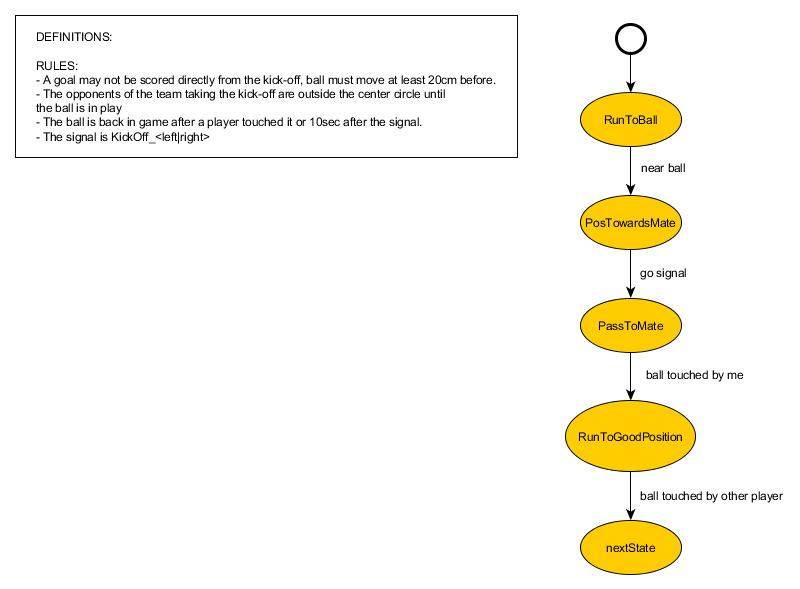
\includegraphics[width=\textwidth]{Grafiken/KI/Standardsituationen/KickoffSM}
	\caption{Spezialrolle - Kickoff}
	\label{fig:Standard - Kickoff}
\end{figure}

Der Ansto{\ss} besteht generell aus einer Positionierung am Ball mit anschließendem Pass. Es ist darauf zu achten die Spielregel für den Ansto{\ss} nicht zu verletzen. Nachdem der Ball berührt wurde, darf der gleiche Spieler diesen nicht erneut berühren. Deshalb wird hier nach dem Pass eine Neupositionierung vorgenommen und somit versucht dem Ball aus dem Weg zu gehen.\\
\\
Benötigte Behaviors sind KickToPosition und RunToPosition. Eine Logik für die Positionierung am Ball muss ebenso wie die Neupositionierung vorhanden sein.\\
\\
Es wurde hier der Pass gewählt, da der uns zur Verfügung stehende Kick leider nicht weit genug kommt, als dass sich ein Kick in die gegnerische Hälfte lohnen würde. In Turnieren sieht man häufig einen direkten Kick weit in die gegnerische Hälfte, was vermutlich die bessere Strategie ist wenn der Kick 10+ Meter weit kommt.

\subsubsection{Freisto{\ss}, Ecke}
\textit{Verfasser: Stumpf}\\
\\
\begin{figure}[H]
	\centering
	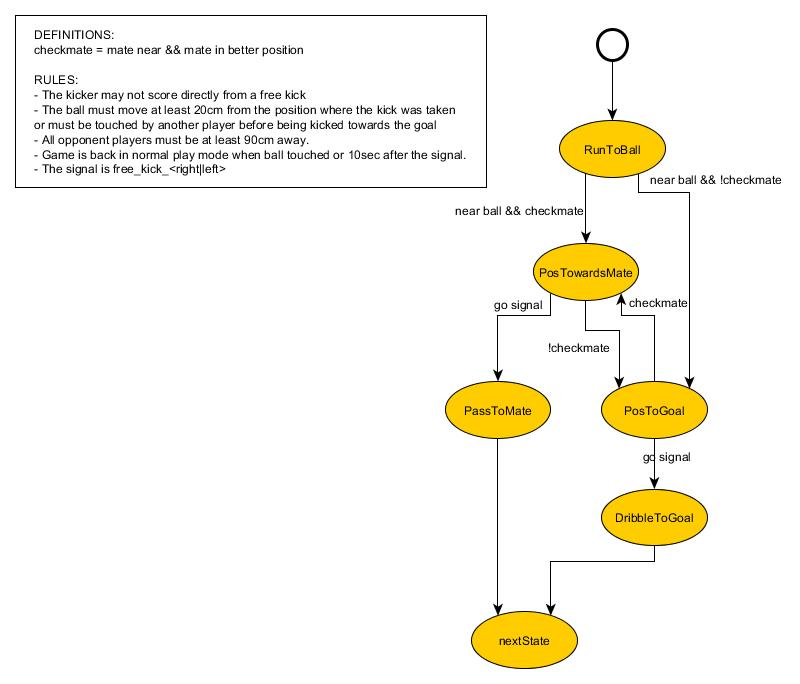
\includegraphics[width=\textwidth]{Grafiken/KI/Standardsituationen/FreeKickSM}
	\caption{Spezialrolle - Freekick}
	\label{fig:Standard - Freekick, Cornerkick}
\end{figure}

Vorweg zu erwähnen ist, dass der Freisto{\ss} aus dem aktuellen Regelwerk (Stand: 2015) entfernt und durch Auszeiten ersetzt wurde. Insofern ist diese Implementierung nur der Vollständigkeit und Kompatibilität halber aufgeführt.\\
\\
Da beim Freisto{\ss} kein direktes Tor erzielt werden darf wird hier einfach zum nächsten Mitspieler in der Nähe gepasst, sollte kein Mitspieler in der Nähe sein, der in einer besseren Position als man selbst ist, so wird in Richtung Tor gedribbelt.\\
\\
Benötigte Behaviors sind KickToPosition, RunToPosition sowie DribbleBall. Es wird eine Logik für die Positionierung vorausgesetzt.\\
\\
Als Zustandsautomat für die Standardsituation Ecke wurde der selbe verwendet wie für den Freisto{\ss}.

\subsubsection{Einwurf}
\textit{Verfasser: Stumpf}\\
\\
\begin{figure}[H]
	\centering
	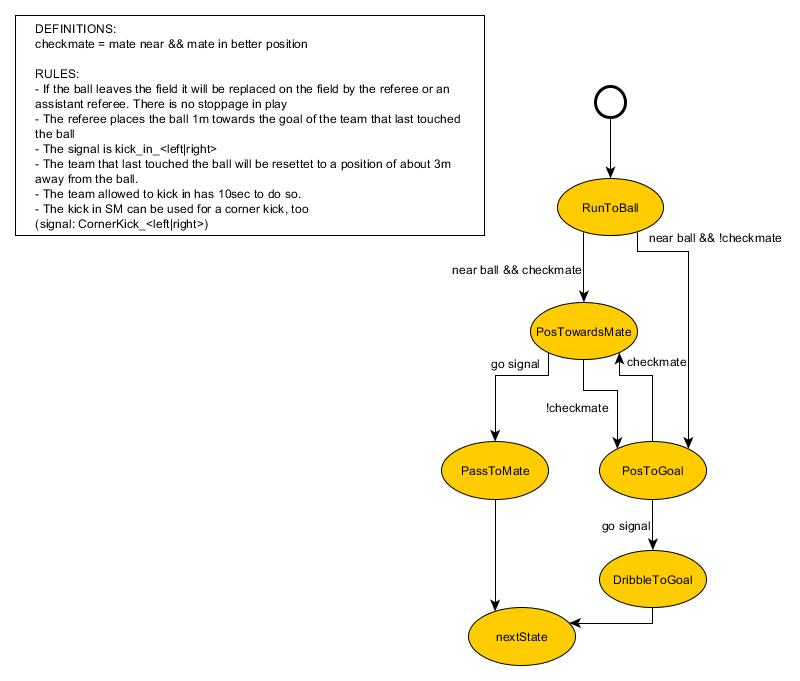
\includegraphics[width=\textwidth]{Grafiken/KI/Standardsituationen/KickInSM}
	\caption{Spezialrolle - Kick in}
	\label{fig:Standard - KickIn}
\end{figure}

Der Zustandsautomat des Einwurfs ist grundsätzlich gleich dem des Freisto{\ss}es, da nicht geworfen, sondern gekickt wird.

\subsubsection{Absto{\ss}}
\textit{Verfasser: Stumpf}\\
\\
\begin{figure}[H]
	\centering
	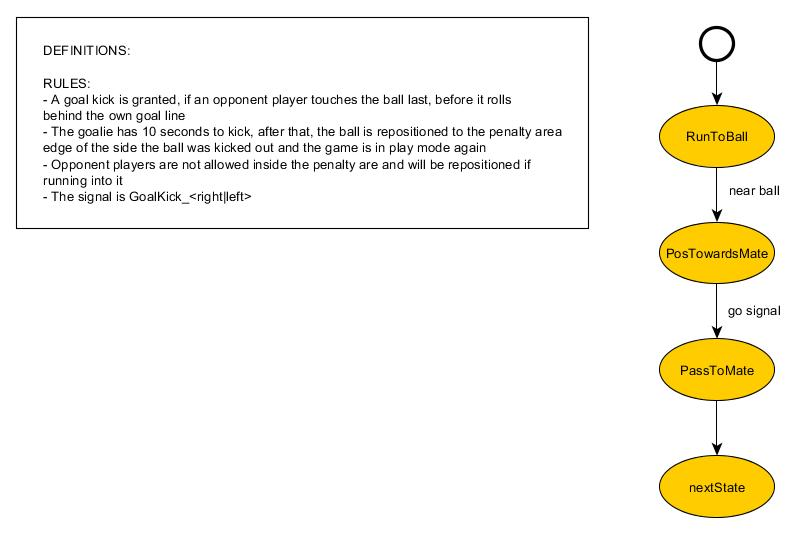
\includegraphics[width=\textwidth]{Grafiken/KI/Standardsituationen/GoalKickSM}
	\caption{Spezialrolle - Goalkick}
	\label{fig:Standard - Goalkick}
\end{figure}

Der Zustandsautomat des Absto{\ss}es ist grundsätzlich gleich dem des Ansto{\ss}es. Der einzige Unterschied ist, dass der Ball nach einem Abstoß erneut berührt werden darf, weshalb die Neupositionierung und Vermeidung der Ballberührung wegfällt.

\subsubsection{Implementierung}
\textit{Verfasser: Stumpf}\\
\\
Bei der Implementierung der Standardsituationen wollte ich unnötige Redundanz vermeiden. Die Rollen waren sich so ähnlich, dass ich mich entschlossen habe, sie auf gemeinsamen States aufzubauen.\\
\\
Die beiden gemeinsam verwendeten States sind InteractWithBall und MoveToBall.\\
\\
Solange man sich nicht in der Nähe des Balles befindet wird man sich im State \textbf{MoveToBall} aufhalten. Dieser State gibt intern eine RunToPosition Behavior zurück, mit dem Ziel sich in die Nähe des Balls zu begeben.\\
\\
Ist man in der Nähe des Balls, so wird man in den \textbf{InteractWithBall} State wechseln. Dieser enthält die meiste Logik und entscheidet wie mit dem Ball interagiert werden soll.\\ 
Intern wird zuerst entschieden, welche Interaktion ausgeführt werden soll. Zur Auswahl stehen:
\begin{itemize}
\item Zum Tor Dribblen
\item Zum Tor Schießen
\item Zu Mitspieler passen
\end{itemize}
Die Interaktionen sind über eine Methode des States \\
\\
\texttt{public void setActiveInteractions(\\boolean dribbleToGoal, boolean passToMate, boolean kickToGoal)}\\
\\
konfigurierbar. Es wird nur aus aktiven Interaktionen ausgewählt.
Die Entscheidung wird getroffen anhand von gemeinsamer Logik, zum Beispiel \textit{\glqq Befinde ich mich in der Nähe des Tors, so dass ein Torschuss erfolgreich sein könnte?\grqq}, oder \textit{\glqq Ist ein Mitspieler in der Nähe, der besser steht als ich?\grqq}.

\section{Grafisches Debugging}\label{se:Grafisches Debugging}
\textit{Verfasser: Schramm}\\
\\
Nach einer kurzen Einarbeitung in Simspark und der Verwendung der ersten Frameworks, wurde klar, dass weder ein klassisches Logging, noch Debugging ausreichende Möglichkeiten bieten um eine schnelle Entwicklung zu ermöglichen. Durch Logging kann zwar der interne Ablauf nachvollzogen werden, jedoch sind serialisierte, dreidimensionale Vektoren wenig anschaulich.
Ein Debugging mit Breakpoints stört die Synchronisierung mit den Serverzyklen und ist somit noch eingeschränkter nutzbar. Deshalb wurde nach anderen Möglichkeiten der Analyse gesucht.

\subsection{RoboViz}
\label{subsec:RoboViz}
\textit{Verfasser: Schramm}\\
\\
Der zusätzliche Monitor: 'RoboViz' ist ein Werkzeug, das genau für diesen Zweck entwickelt wurde. Er dient als Ersatz für den Standardmonitor von Simspark und ermöglicht ein zeichnen von zusätzlichen Informationen, direkt in der 3D-Szene. So können über geometrische Primitive und Textausgaben bei der Steuerung der NAOs anfallende Daten ausgeben werden. Dies geschieht in einer visuell schnell erfassbaren Weise, sodass Vektorumrechnungen oder -vorstellungen vermieden werden.\\

Der RoboViz nimmt über ein UDP-Socket die Debuginformationen in einem eigen Bytearray-Format entgegen. Die Befehle variieren in ihrer Länge, so nimmt eine Linie mehr Bytes entgegen, als ein Punkt. Gemein ist jedoch allen Befehlen, das diese mit einem 'set name' und einem Nullbyte abgeschlossen werden. Zu beachten ist, dass alle eingehenden Anweisungen mit dem selben 'set name' zunächst gesammelt werden. Erst nach einem 'swap buffer' Befehl werden alle diese gezeichnet. Sie sind solange sichtbar, bis der nächste 'swap buffer' eingeht.\\
Die mitgelieferte Java-Bibliothek ersetzt die Bytecodierung durch Methodenaufrufe mit entsprechenden Parametern.

\begin{figure}[H]
	\centering
	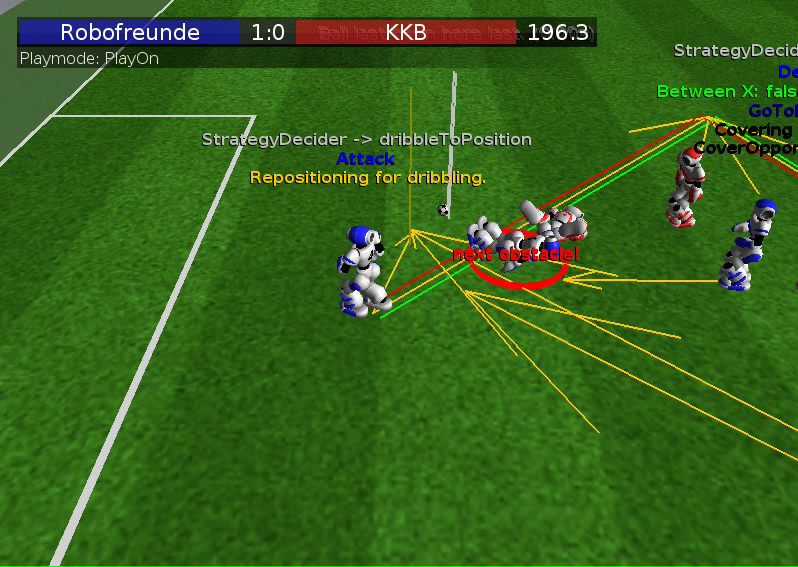
\includegraphics[width=\ScaleIfNeeded]{Grafiken/RoboViz/RoboVizzingToDaMax}
	\caption{Visualisierungen im Endspiel}
	\label{fig:roboviz-endgame}
\end{figure}


\subsection{Debugger}
\label{subsec:Debugger}
\textit{Verfasser: Schramm}\\
\\
Um die Handhabung für die Entwicklung im Magma-Framework zu vereinfachen, wurde eine Debugger Schnittstelle geschaffen. Diese kapselt die Verwaltung der 'set name's sowie Farbcodes und konvertiert die Magma-typischen Vector3D-Elemente in die benötigten Parameter. Eine typische Ausgabe, wie sie beispielsweise beim Dribbeln erzeugt wird, wird so auf wenige Zeilen eingedampft:
\begin{lstlisting}[caption=RoboVizDebugger, captionpos=b, label=lst:Debug]
if (!getDebugger().isHidden()) {
   getDebugger().drawString("Repositioning for dribbling.", RoboVizColors.ORANGE);
   getDebugger().drawVector(getMyPosition(), dribbleStartPosition, RoboVizColors.ORANGE);
}
\end{lstlisting}

Zudem bietet der Debugger die Möglichkeit einen weiter abzuleiten, der dessen Socket mitverwendet und gleichzeitig einen eigenen 'set name' bekommt. Über Letzteren kann zur Laufzeit im RoboViz-Monitor die Ausgabe unterdrückt werden, ohne dass dies den ursprünglichen Debugger beeinflusst.

\begin{figure}[H]
	\centering
	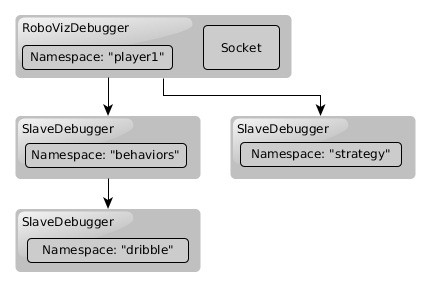
\includegraphics[width=240pt]{Grafiken/RoboViz/Debugger}
	\caption{Debugger - Beispiel-Hierarchie}
	\label{fig:debugger-hierarchy}
\end{figure}

Die entsprechen Klassen befinden sich in 'srcCommon/visualization'.

\subsection{Verteilung}
\label{subsec:Debugger Verteilung}
\textit{Verfasser: Schramm}\\
\\
Um die Hierarchie der Debugger richtig aufzubauen, werden diese über ein 'Debuggable' Interface verteilt. Der Basis-Debugger wird in der Factory-Klasse der RoboFreunde erzeugt und dann an alle 'Behaviors' und 'DecisionMakers' verteilt, die das Interface implementieren. Daher ist es zum Debuggen notwendig das 'NaoRF'-Modell zu verwenden oder sich selbst um die Verteilung zu kümmern.\\
Wird kein Basis-Debugger erstellt, greifen die 'Debuggables' auf einen NullDebugger zurück, der standardmäßig versteckt ist und somit die anfallende Rechenlast minimiert.\\
Ein derartige, nachträgliches Verknüpfen der Komponenten außerhalb der Konstruktoren ermöglicht auch eine abwärts Kompatibilität zu anderen MetaModellen, die von RoboViz keine Ahnung haben.

\subsection{Debugger Graph}
\label{subsec:Debugger Graph}
\textit{Verfasser: Schramm}\\
\\
Für eine einfachere Auswertung von Messwerten wurde eine Graph-Klasse erzeugt, die eine Reihe von Messwerten als Liniendiagramm darstellt. Beim Erstellen wird ein Ort für den Ursprung und ein Vektor, der sowohl Orientierung als auch Größe des Graphen festlegt übergeben. Ein übergebener Debugger dient als Ziel für alle Zeichenoperationen. Zum Darstellen der Daten können diese als Liste von Vector2D-Elementen übergeben werden. Die Skalierung der Achsen erfolgt automatisch und passt sich gegebenenfalls neuen Werten an. (Negative Werte sind ungetestet)\\
Der Graph sieht nicht nur toll aus und vereinfacht die Aufnahme von vielen Meßwerten für den Menschlichen Geist, er demonstriert auch eindrucksvoll wie Leistungsstark der RoboViz-Monitor bei der Darstellung auch sehr vieler Elemente ist.

\begin{figure}[H]
	\centering
	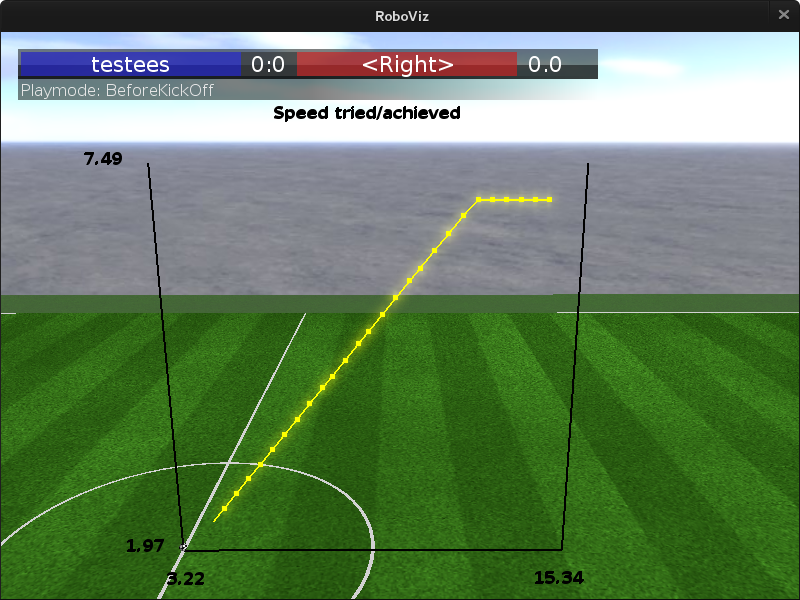
\includegraphics[width=\ScaleIfNeeded]{Grafiken/RoboViz/Graph}
	\caption{Debugger - Graph}
	\label{fig:debugger-graph}
\end{figure}

\section{Manuelle Steuerung}\label{se:Manuelle Steuerung}
\textit{Verfasser: Schramm}\\
\\
Um die KI interaktiv zu testen, wurde eine Möglichkeit integriert, den Nao zu beeinflussen und seine Reaktion beobachten. Dabei unterscheidet man zwei Szenarien:
\begin{itemize}
\item Einen Nao durch einen zweiten, manuellen stören.
\item Einen Nao manuell in eine Situation bringen, danach die KI übernehmen lassen.
\end{itemize}

\subsection{Aufbau}
Dazu wurde ein DecisionMaker für manuelle Steuerung implementiert. Dieser ersetzt die KI und nimmt Befehle von einem manuellen Controller entgegen.
Um eine direkte Steuerbarkeit zu gewährleisten werden einige Befehle in einer Queue gesammelt und abgearbeitet.

Neben den primären Befehlen, die in jedem Server-Zyklus abgearbeitet werden, wie zum Beispiel: Laufen, Kicken, Aufstehen … existieren auch Befehle, die parallel zu diesen ausgeführt werden können. Diese umfassen Sprechsignale und Kopfdrehungen. Sie sind in ihrer Funktion disjunkt zu den Körperbefehlen was die verwendeten Gelenke angeht. Würden diese in der Befehlsqueue ausgeführt werden, käme es zu einer Verzögerung der primären Befehle um die entsprechenden Zyklen. Deshalb werden sie in einer extra Queue für außerordentliche Befehle gesammelt und direkt vor der ordentlichen Queue ausgeführt.\\
Die zugehörigen Klassen befinden sich im Package:\\ \texttt{magma.agent.decision.simple.manual}.

\subsection{Autopiloten}
Um die Übernahme der Kontrolle durch eine KI zu ermöglichen, werden bestehende KIs als Autopiloten eingebunden. Jeder Autopilot beinhaltet einen DecisionMaker der in regulären Bots verwendet wird. Über den manuellen Controller kann nun zwischen den Autopiloten gewechselt werden. Wird ein solcher dann aktiviert, gibt der Controller einen delegierenden Befehl an den Manuellen DecisionMaker weiter. Dieser Befehl übergibt alle Entscheidungen intern an den ihm zugeordneten KI-DecisionMaker. Somit wird der Bot von der KI übernommen. Soll zur manuellen Steuerung zurückgekehrt werden, wird der Befehl auf erledigt gesetzt und somit vom manuellen DecisionMaker aus der Queue entfernt.\\
Die verwendeten Autopiloten werden im Konstruktor übergeben. Die Auswahl erfolgt in der ComponentFactory unter \texttt{magma.agent.general}. Zur einfacheren Übersicht wurde eine Vorauswahl in einer Methode 'getAutoPilots(...)' ausgelagert.

\begin{figure}[H]
	\centering
	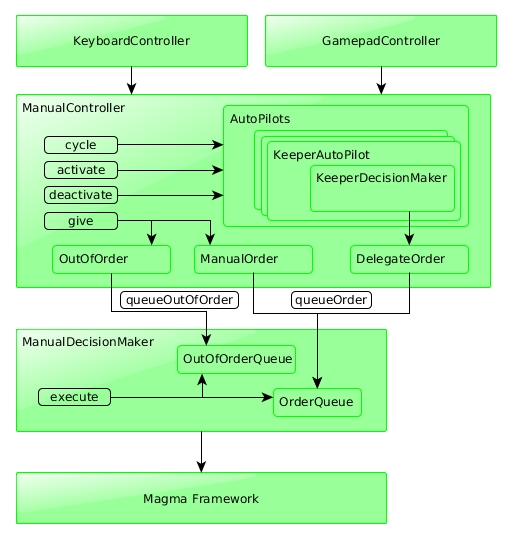
\includegraphics[width=\ScaleIfNeeded]{Grafiken/ManualCtrl/ManualDecisionMaker}
	\caption{ManualDecisionMaker}
	\label{KickMetrikAgent}
\end{figure}

\subsection{Keyboard Controller}
Eine Implementierung des Controllers stellt die Keyboardvariante dar. Dabei werden sämtliche Tastatureingaben über ein awt-Fenster abgefangen und ausgewertet. Durch drücken der Pfeiltasten lässt sich der NAO beispielsweise in die Verschiedenen Richtungen navigieren.\\
Um diesen Controller auszuwählen wird in den Startparametern die DecisionMakerID 100 übergeben.

\begin{figure}[H]
	\centering
	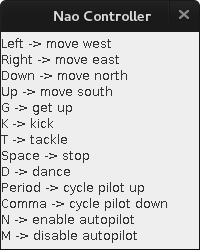
\includegraphics[width=160pt]{Grafiken/ManualCtrl/KeyboardController}
	\caption{KeyboardController - Fenster}
	\label{fig:keyboardcrtl}
\end{figure}


\subsection{Gamepad Controller}
Für eine feinere Steuerung wurde eine Schnittstelle für Gamepads integriert. Diese bietet die selben Möglichkeiten wie über Tastatur. Dabei wurden für einige gängige Controller bereits Profile angelegt. Um diese zu erweitern und eigene hinzuzufügen, muss in der Klasse GamepadController ein neue Initialisierung angelegt werden, die das entsprechende Tastenmapping umsetzt (siehe Beispiel).\\
Um diesen Controller auszuwählen wird in den Startparametern die DecisionMakerID 101 übergeben.

\begin{lstlisting}[caption=InitializeGamePad, captionpos=b, label=lst:Gamepad]
private void initializeXBox() {
    commandMap.put("B", this::orderGetUp);
    commandMap.put("A", this::orderKick);
    commandMap.put("X", this::orderPush);
    commandMap.put("Y", this::orderStop);
    commandMap.put("Start", this::orderDance);
    commandMap.put("Right Thumb", this::cycleAutoPilotUp);
    commandMap.put("Left Thumb", this::cycleAutoPilotDown);
    commandMap.put("Mode", this::toggleAutoPilot);
    commandMap.put("Select", this::toggleEgoWalk);
    walkXComponent = Component.Identifier.Axis.X;
    walkYComponent = Component.Identifier.Axis.Y;
    lookXComponent = Component.Identifier.Axis.RX;
    lookYComponent = Component.Identifier.Axis.RY;
}
\end{lstlisting}

\section{Strategien}
\textit{Verfasser: Weber}\\
\\
Das Konzept einer Strategie wurde bereits im Kapitel \ref{StrategienLabel} besprochen. Der folgende Abschnitt widmet sich der Implementierung sowie Konfiguration.

\subsection{Implementierung}
\textit{Verfasser: Weber}\\
\\
Im Konzept werden unterschiedliche Strategien erw"ahnt. Aus Zeitgr"unden konnte jedoch nur eine echte Strategie entwickelt werden. Es ist zwar eine aggressive sowie defensive Strategie vorhanden, diese unterscheiden sich jedoch nicht in ihrer Logik. Deswegen wird im folgenden Text nur von der Strategie gesprochen. Die Strategie unterscheidet nach Haupt- und Spezial-Rollen, die nach Bedarf gew"ahlt werden.

\begin{itemize}

\item Hauptrolle
\begin{itemize}
\item Torwart
\item Verteidiger
\item Mittelfeld
\item St"urmer
\end{itemize}

\item Spezialrollen
\begin{itemize}
\item Beam
\item Ecke
\item Freisto"s
\item Einwurf
\item Ansto"s
\item Party

\end{itemize}
\end{itemize}

Ein Roboter darf in dieser Strategie blo"s eine Hauptrolle annehmen, jedoch beliebig viele Spezialrollen besitzen.\\

\begin{lstlisting}[caption=Entscheidung zu einer Rolle, captionpos=b, label=EntscheidungRolleStrategie]
if(gameState != lastState) {
    decided = true;
    lastState = gameState;

    switch (gameState) {
        case OWN_GOAL:
        case OPPONENT_GOAL:
        case BEFORE_KICK_OFF:
            currentRole = beam;
            break;
        case OWN_CORNER_KICK:
            currentRole = resolveSecondary(Roles.CornerKick);
            break;
        case OWN_FREE_KICK:
            currentRole = resolveSecondary(Roles.FreeKick);
            break;
        case OWN_GOAL_KICK:
            currentRole = resolveSecondary(Roles.GoalKick);
            break;
        case OWN_KICK_OFF:
            currentRole = resolveSecondary(Roles.KickOff);
            break;
        case GAME_OVER:
            currentRole = party;
            break;
        case PLAY_ON:
            currentRole = resolveMainRole();
            break;
    }

    if(currentRole != null) {
        currentRole.init(getPlayer());
        currentRole.setDebugger(getDebugger());
    }
}
\end{lstlisting}

Aus dem abgebildeten Quelltext lassen sich folgende Funktionalit"aten ableiten. Der "Ubergang zu einer neuen Rolle findet nur statt, wenn ein Wechsel des GameState stattgefunden hat. Es kann ebenfalls zu dem Fall kommen, dass die aktuelle Rolle nicht gesetzt wurde, daf"ur wurde der Null-Check nach der Switch implementiert. Sollte der Einsatz von einer Spezialrolle notwendig werden, wird nur der n"aheste Roboter aktiv. Dies wird auch durch ein Blick in die \lstinline$resolveSecondary$ Methode best"atigt.\\
\\
\begin{lstlisting}[caption=resolveSecondary Methode der Strategie, captionpos=b, label=EntscheidungRolleStrategie]
private BotState resolveSecondary(Roles role) {
    current = role;
    List<Roles> secondary = availableRoles.stream()
        .filter(roles -> (roles.isSecondaryRole()))
        .collect(Collectors.toList());

    if(secondary.stream().anyMatch(roles -> roles == role) && nearestPlayer()) {
        switch (role) {
            case CornerKick:
                return corner;
            case FreeKick:
                return free;
            case GoalKick:
                return goal;
            case ThrowIn:
                return throwIn;
            case KickOff:
                return kickOff;
        }
    }

    current = Roles.Null;
    return nullBot;
}
\end{lstlisting}

\subsection{Konfigurierung}
\textit{Verfasser: Weber}\\
\\
Zur Konfiguration wurden Java Virtual Machine (JVM) Properties verwendet. Diese werden beim Start der JVM als Konsolenparameter mit dem Prefix '-D' angegeben und k"onnen anschlie"send innerhalb der JVM mit \lstinline$System.getProperty("key", "fallback");$ abgerufen werden. Die gew"unschten Rollen f"ur den aktuellen Spieler m"ussen mit dem Schl"ussel ``playableRoles'' angegeben werden. Die einzelnen Rollen lauten:

\begin{itemize}
\item Keeper
\item Defense
\item Middle
\item Attack
\item CornerKick
\item FreeKick
\item GoalKick
\item ThrowIn
\end{itemize}

Es wurde zu dieser Art der Konfiguration gegriffen, um eine feste Verdrahtung von Rollen im Quelltext zu vermeiden. Außerdem ist damit eine feingranulare Einstellung sowie flexibles "Andern von Rollen m"oglich.

\section{Strategie-Entscheider}
\textit{Verfasser: Weber}\\
\\
Das Konzept des Strategie-Entscheider wurde bereits in Kapitel \ref{StrategieEntscheiderLabel} besprochen. Der folgende Abschnitt zeigt seine Implementierung.\\

Der aktuelle Entscheider arbeitet mit insgesamt 3 unterschiedlichen Strategien, wobei es sich um eine einfache Proof of Concept-Strategie handelt, sowie die aus den Vorg"anger bekannten defensiver und aggressiver Strategie. Die simple Strategie kann nur "uber einen JVM Parameter aktiviert werden, sollte dieser nicht gesetzt sein, wird die Logik f"ur die aggressive, bzw. defensive Strategie ausgef"uhrt. Wie im folgenden Code Ausschnitt gezeigt, findet eine Transistion von defensive zu aggressive Strategie statt, sobald sich das eigene Team in einem 2 Punkte R"uckstand befindet.

\begin{lstlisting}[caption=Interne Logik des Strategie-Entscheiders, captionpos=b]
if (USE_SIMPLE) {
    currentStrategy = simple;
    currentStrategy.init(getPlayer());
} else {
    int ownGoalCount = getPlayer().getModel().getWorldModel().getGoalsWeScored();
    int otherGoalCount = getPlayer().getModel().getWorldModel().getGoalsTheyScored();
    PossibleStates newState;

    if (ownGoalCount + 2 <= otherGoalCount) {
        currentStrategy = aggressive;
        newState = PossibleStates.Agressive;
    } else {
        currentStrategy = defensive;
        newState = PossibleStates.Passive;
    }

    //Call Init, only when State has changed.
    if (newState != oldState) {
        currentStrategy.init(getPlayer());
    }

    oldState = newState;
}

currentStrategy.update();
\end{lstlisting}

\section{Zusammenfassung und Ausblick}
\textit{Verfasser: Weber}\\
\\
Zusammenfassend kann man sagen, dass ein zufriedenstellendes Ergebnis erzielt werden konnte, obwohl die Aufgabenstellung einen komplizierten Sachverhalt darstellt und das Team zum Start gro"se Probleme hatte. Die grundlegenden Aktionen, die ein Roboter ausf"uhren kann, funktionieren mit den selbst entwickelten Verbesserungen fast ohne Zwischenf"alle, was sich auch positiv auf die Kicking/Time Challenge ausgewirkt hat. Es existiert eine breite Vielfalt von unterschiedlichen Rollen, die sich Dank der Flexibilit"at der zugrundeliegenden Architektur einfach realisieren ließen. Die entwickelten M"oglichkeiten zum Debugging und Testen der Roboter hatten ebenfalls einen gro"sen Einfluss auf den Erfolg des Projekts.\\
\\
Die Wahl des Frameworks Magma-Offenburg und damit für die Programmiersprache Java, hat sich als Vorteilhaft erwiesen. Bef"urchtungen, dass die JVM nicht performant genug sei, konnten nicht beim Abschluss Turnier und dem Testspielen beseitigt werden.\\
\\
F"ur zuk"unftige Semester l"asst sich zusammenfassend sagen, dass es sich hierbei um eine durchaus erf"ullbare Aufgabe handelt. Die unteranderem ma"sgeblich davon beeinflusst wird, welches Framework zu Beginn gew"ahlt wird.
\section{Verzeichnisse}
\listoffigures

\lstlistoflistings
\printbibliography

\begin{appendices}
\section{Use cases für den Bot ``Mittelfeldspieler''}
\label{usecases_midfielder}

\noindent\makebox[\textwidth]{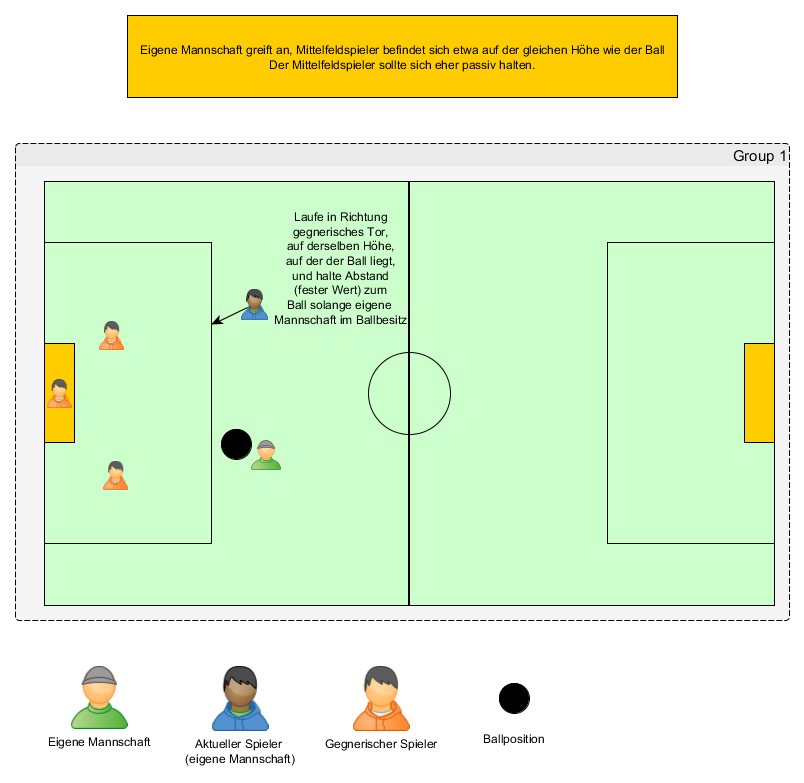
\includegraphics[angle=90,origin=c,width=0.9\paperwidth]{Grafiken/KI/mittelfeldspieler/eigene_mannschaft_im_angriff.png}}

\noindent\makebox[\textwidth]{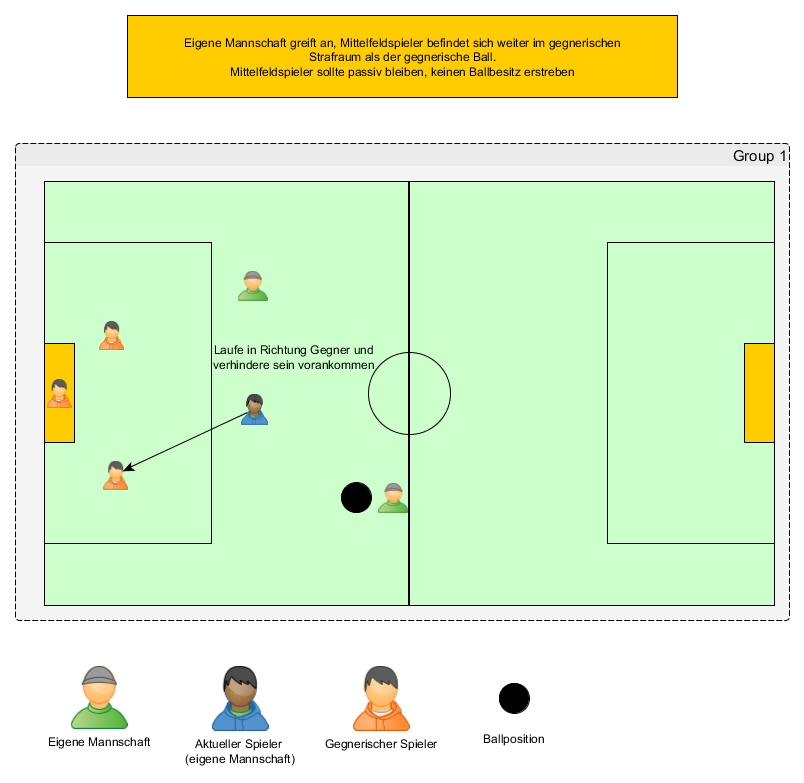
\includegraphics[angle=90,origin=c,width=0.9\paperwidth]{Grafiken/KI/mittelfeldspieler/eigene_mannschaft_im_angriff_fall_2.png}}

\noindent\makebox[\textwidth]{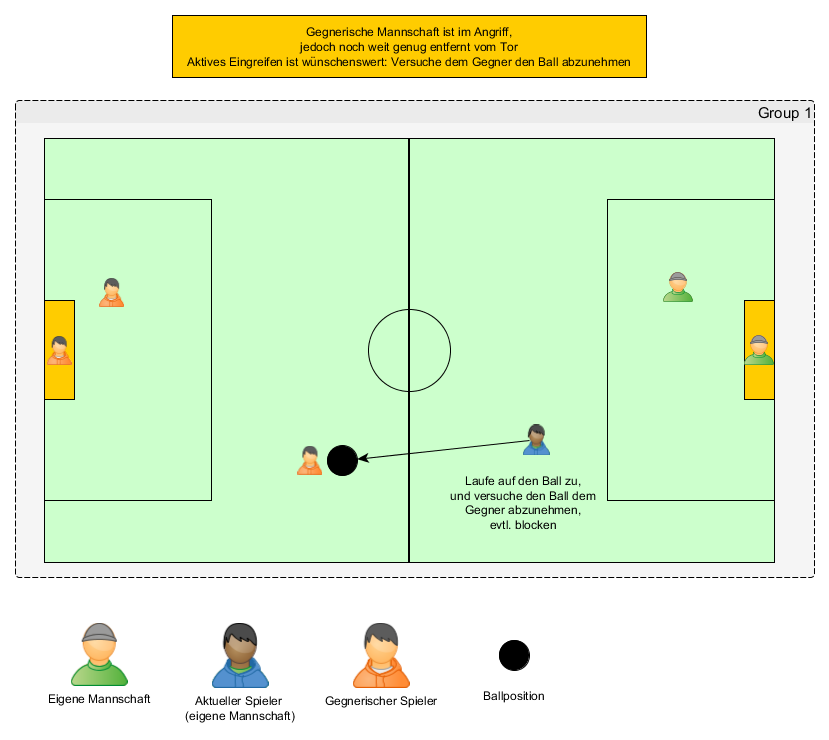
\includegraphics[angle=90,origin=c,width=0.9\paperwidth]{Grafiken/KI/mittelfeldspieler/gegnerische_mannschaft_im_angriff.png}}

\noindent\makebox[\textwidth]{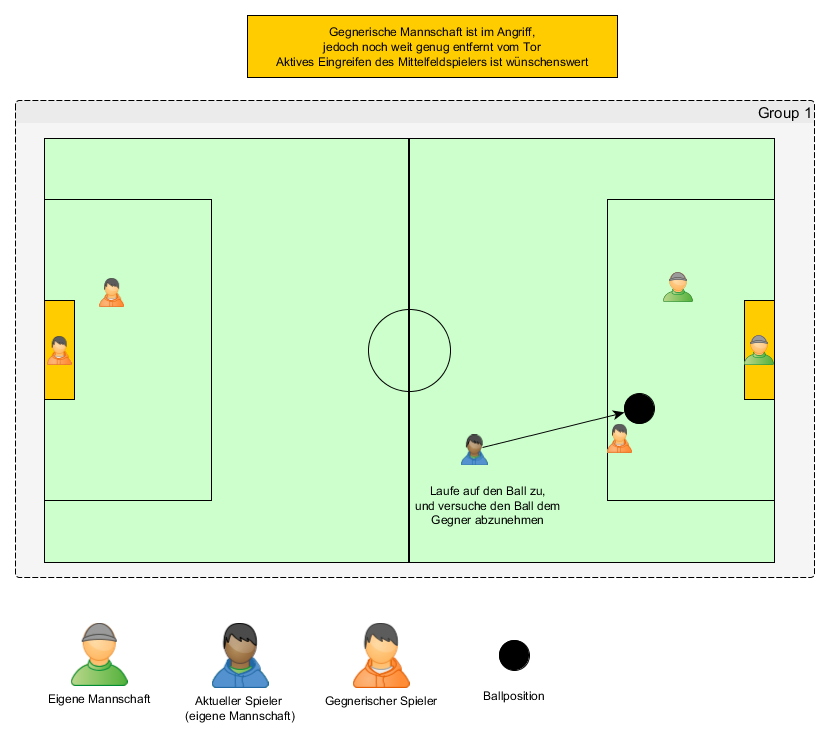
\includegraphics[angle=90,origin=c,width=0.9\paperwidth]{Grafiken/KI/mittelfeldspieler/gegnerische_mannschaft_im_angriff_fall_2.png}}

\section{Zustandsdiagramm für den Bot ``Mittelfeldspieler''}
\label{statechart_midfielder}

\noindent\makebox[\textwidth]{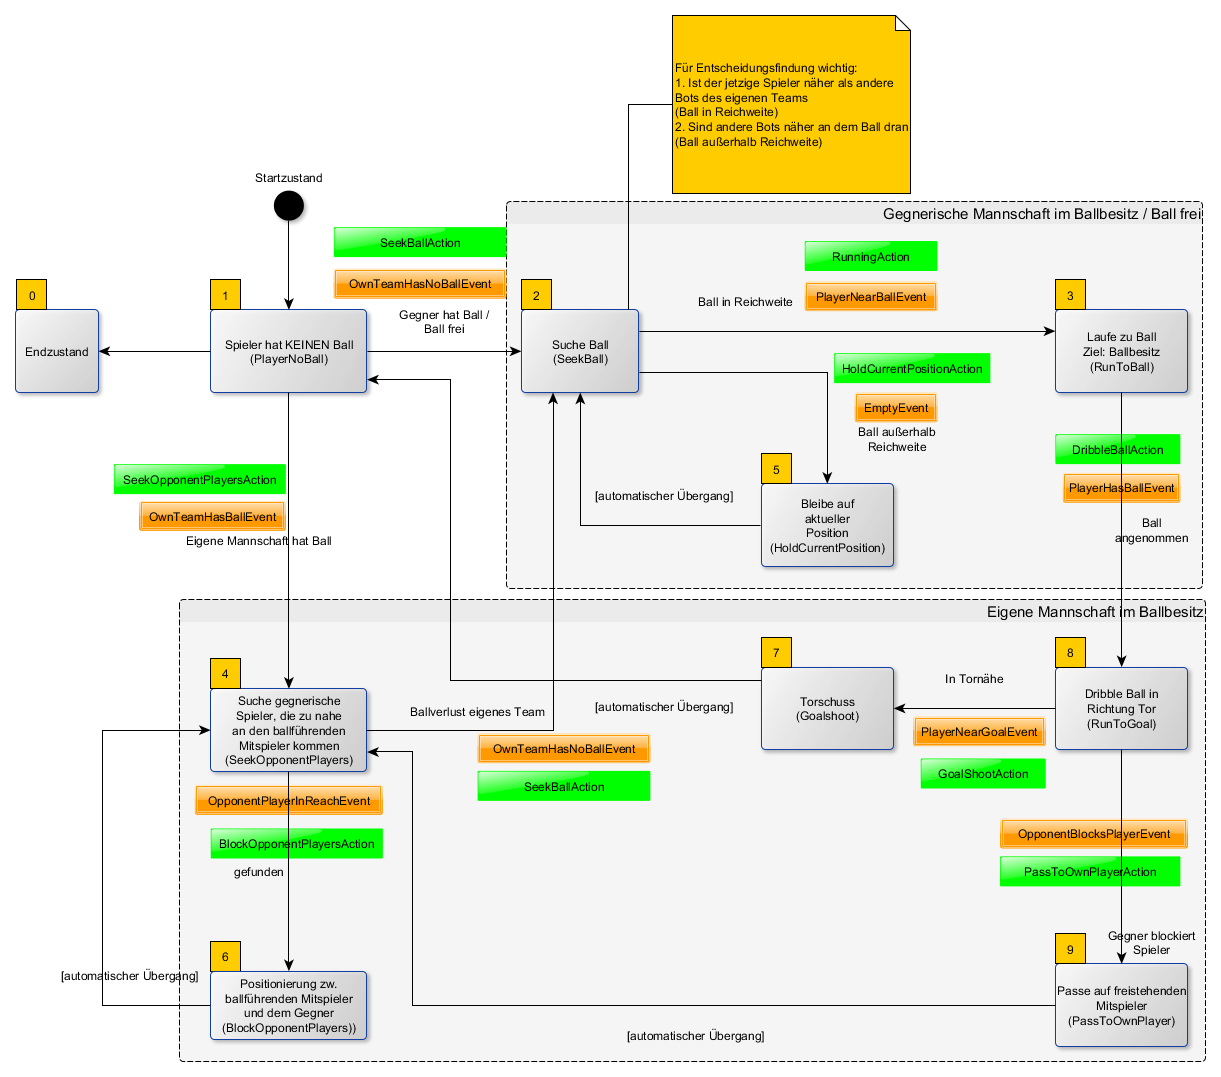
\includegraphics[angle=90,origin=c,width=0.9\paperwidth]{Grafiken/KI/mittelfeldspieler/mittelfeldspieler.png}}

\end{appendices}

\end{document}